\documentclass[french]{article}


\usepackage[utf8]{inputenc} % encode en UTF8

\usepackage[T1]{fontenc}





\usepackage[top=2cm, bottom=2cm, left=3cm, right=3cm]{geometry}
\usepackage{graphicx}
\usepackage{caption}
\usepackage{subcaption}
\usepackage{float}
\graphicspath{ {./photo/} }

%Belles fraction de fration \cfrac
\usepackage{amsmath}

\usepackage{tikz}
\usepackage{circuitikz}

\parindent=0cm 

\usepackage{listings}             % Include the listings-package

\lstset{language=Matlab}          % Set your language (you can change the language for each code-block optionally)


%
%\lstdefinestyle{CStyle}{
%	backgroundcolor=\color{backgroundColour},
%	commentstyle=\color{mGreen},
%	keywordstyle=\color{magenta},
%	numberstyle=\tiny\color{mGray},
%	stringstyle=\color{mPurple},
%	basicstyle=\footnotesize,
%	breakatwhitespace=false,
%	breaklines=true,
%	captionpos=b,
%	keepspaces=true,
%	numbers=left,
%	numbersep=5pt,
%	showspaces=false,
%	showstringspaces=false,
%	showtabs=false,
%	tabsize=2,
%	language=C
%}

\input{titre}


\begin{document}
\myTitle[Rapport de mini-projet \\ - Électronique Hautes Fréquences - ]
\newpage

\tableofcontents
\newpage
\listoffigures
\listoftables
\newpage


\vspace*{4cm}
\section*{Résumé}
L'électronique des hautes fréquences est une discipline essentielle lorsqu'il s'agit de manipuler et modifier des signaux dont la longueur d'onde est de l'ordre des dimensions du circuit.\\
Et ce domaine est d'autant plus indispensable dans un monde connecté dont les produits électroniques tendent à être toujours plus rapides. Cette discipline est présente dans le domaine des télécommunications que ce soit civil ou militaire, dans le médical ou encore la sécurité et regroupe un ensemble de problématique comme l'émission ou réception de signaux, leur traitement par filtrage ou amplification et bien plus encore.\\
Ce rapport permet de découvrir une infime branche de l'électronique hautes-fréquences, et se focalise sur la découverte de la technologie micro-ruban et la conception selon un cahier des charges de diverses fonctions d'électronique.

\vspace{1cm}

\section*{Remerciement}
Nous souhaitons sincèrement remercier Yann MAHE pour le temps et la patience dont il fait preuve pour nous enseigner sa discipline. Il a su s'adapter en corrigeant nos lacunes tout en évoquant des notions nouvelles issues de la recherche et à aiguiser davantage notre curiosité sur le domaine des hautes-fréquences.\\
Nous remercions tout autant Anne CHOUSSEAUD qui, durant les travaux pratiques, nous a accompagnée avec calme et passion.\\
Et pour n'oublier personne, nous sommes reconnaissant envers Tchanguiz RAZBAN pour les cours dispensés et les ressources pédagogiques mises à dispositions.\\
Un merci à notre camarade Huanqing LIN qui nous a aidé pour la partie amplification.

\newpage
\pagestyle{plain} % Début de la numérotation des pages

\section{Introduction}
\subsection{Contextualisation}
La formation ETN (Électronique et technologies numériques) offerte par l'école polytechnique de l'Université de Nantes propose d'aborder diverses branches de l'électronique, de la conception de circuits numériques au traitement du signal en passant par l'électronique analogique des hautes-fréquences. Tous les domaines étudiés au cours de cette formation apportent tous les outils nécessaires à l'ingénieur en électronique.\\
Ce rapport porte sur la matière électronique des hautes-fréquences. Il s'agit d'une toute nouvelle discipline venant bousculer le monde de l'électronique connu par l'analogique basses fréquences étudié en 3ème année de cycle ingénieur. Une telle matière permet d'aborder la manipulation de signaux de fréquences élevées, à tel point que les longueurs d'ondes mises en jeu sont proches des dimensions géométriques du circuit.\\
Ce rapport de travaux pratiques s'inscrit dans une application concrète du monde de l'ingénierie, c'est-à-dire la conception d'une solution répondant à une problématique, et cela selon un cahier des charges.\\

\subsection{Objectifs du mini-projet}
Ce rapport vise à combiner la théorie et la pratique de la matière électronique des hautes-fréquences. Chaque partie analysera d'abord en détail les principes appliqués et les méthodes utilisées. Des logiciels de modélisation et de simulation comme ADS, AppCAD ou encore GNU Octave seront utilisés pour mettre ces principes en application.\\

\noindent Les autres objectifs sont donnés ci-dessous :\\

\begin{itemize}
	\item Améliorer la maîtrise des outils de modélisation et de simulation, en particulier d'ADS\\
	\item Découverte de la technologie micro-ruban, son modèle et son cadre de validité\\
	\item Approfondir la compréhension des multiples connaissances acquises au cours du module\\
	\item Permettre d'acquérir plus d'expériences dans la méthodologie de résolution de problèmes et la méthode scientifique
\end{itemize}

\newpage

\section{Étude et caractérisation de la technologie micro-ruban}

\subsection{Avant-propos}

L'électronique des hautes-fréquences consiste en la propagation de signaux à fréquences élevées, et de longueurs d'ondes proches des dimensions du circuit, au travers d'une ligne de transmission. Les lignes de transmissions se déclinent sous diverses familles comme les câbles coaxiaux, les lignes bifilaires, les guides d'ondes ou encore les lignes micro-rubans. Comme le schématise la figure (\ref{fig:modele_microstrip}), une ligne micro-ruban (\textit{microstrip line}) est composée d'un conducteur planaire séparé d'un plan de masse par une couche diélectrique appelée substrat. Une telle technologie a été développée par les laboratoires ITT (\textit{International Telephone and Telegraph}) dans les années 1952. Simple de fabrication et coût bas au regard des autres technologies, la ligne micro-ruban permet la conception de nombreuses fonctions d'électroniques comme le filtrage ou l'amplification.

\begin{figure}[H]
	\centering
	\includegraphics[width=0.8\linewidth]{ressources/modele_microstrip.png}
	\caption{Modèle d'une ligne micro-ruban}
	\label{fig:modele_microstrip}
\end{figure}

Il s'agit dans cette partie de réaliser des caractérisations de lignes, c'est-à-dire la détermination de paramètres d'une ligne micro-ruban. Les lignes à caractériser sont disponibles en laboratoire et sont de l'ordre de quatre, une ligne verre téflon large, verre téflon fin, verre epoxy FR4 large et verre epoxy FR4 fin. Des photographies de ces plaques sont présentes en annexe. Le tableau précisant les dimensions de ces quatre lignes est donné ci-dessous. La caractérisation aura pour finalité l'obtention des paramètres de la ligne telle que la constante diélectrique $\varepsilon_r$ du matériau ainsi que la tangente de perte $\mbox{tan}(\delta)$. Ces paramètres serviront par la suite de valeurs de référence pour la conception de filtres ou d'amplificateurs en technologie micro-ruban. Il s'agit alors de réaliser des mesures à l'aide d'un analyseur de réseau, VNA (\textit{Vector Network Analyzer)}, pour en extraire les valeurs de la matrice $S$. Ces mesures expérimentales constituent la base de la caractérisation. Un modèle théorique de caractérisation de lignes vient se superposer à cette base. Il s'agira alors de faire varier les divers paramètres du modèle afin de faire coïncider celui-ci avec les mesures expérimentales. À ce moment là, les paramètres du modèle correspondent aux paramètres de la ligne et la caractérisation est réussie.


\begin{table}[H]
	\centering
	\begin{tabular}{|c|c|c|c|c|}
		\hline
		Matériaux & Impédance caractéristique & hauteur $h$ & largeur $W$ & longueur $L$\\
		\hline
		Verre téflon large & $Z_C < 50 \Omega$ & 1.58 & 7.87 & 74.82 \\
		\hline
		Verre téflon fin & $Z_C > 50 \Omega$ & 1.58 & 0.469 & 74.978\\
		\hline
		Verre epoxy FR4 large & $Z_C < 50 \Omega$ & 1.50 & 7.928 & 100.037\\
		\hline
		Verre epoxy FR4 fin & $Z_C > 50 \Omega$ & 1.50 & 0.46 & 100.44\\
		\hline
	\end{tabular}
	\caption{Tableau présentant les paramètres géométriques (exprimés en mm) des différentes lignes à caractériser}
	 \label{tab:geo_ligne}
\end{table}

\newpage

\subsection{Présentation du modèle théorique de caractérisation large bande de lignes}

Cette section est consacrée à la présentation d'une structure modélisant le comportement d'une ligne de caractérisation. Un tel modèle possède divers paramètres dont il est nécessaire de déterminer leur valeurs offrant la meilleure superposition avec les courbes expérimentales. Un schéma de ce modèle est présenté ci-dessous. Celui-ci comporte aux extrémités deux terminaux TERM 1 et TERM 2 qui représentent les câbles coaxiaux SMA (\textit{Subminiature version A}) de 50 $\Omega$ du VNA. Les composants MLIN 1 (\textit{Microstrip line 1}), MLIN 2 et 3 sont des lignes micro-rubans de largeur et longueur respectives $W_{acc1}$ et $L_{acc1}$, $W$ et $L$ et $W_{acc2}$ et $L_{acc2}$. MLIN 1 et MLIN 3 modélisent les lignes d'accès et MLIN 2 correspond à la ligne micro-ruban à caractériser. Un tableau ci-dessous précise les différents paramètres.

\begin{table}[H]
	\centering
	\begin{tabular}{|c|c|c|c|c|c|c|}
		\hline
		Matériaux & $W_{acc1}$ & $L_{acc1}$ & $W_{acc2}$ & $L_{acc2}$ & $W$ & $L$\\
		\hline
		Verre téflon large & 4.278 & 5.345 & 4.225 & 5.349 & 7.87 & 74.82 \\
		\hline
		Verre téflon fin & 4.397 & 5.385 & 4.302 & 4.925 & 0.469 & 74.978\\
		\hline
		Verre epoxy FR4 large & 2.918 & 10.031 & 2.944 & 10.063 & 7.928 & 100.037\\
		\hline
		Verre epoxy FR4 fin & 2.862 & 9.982 & 2.914 & 9.948 & 0.46 & 100.44\\
		\hline
	\end{tabular}
	\caption{Tableau présentant les paramètres géométriques (exprimés en mm) des différents MLIN}
\end{table}


\begin{figure}[H]
	\centering
	\input{ressources/schema_modele_caract.tex}
	\caption{Schéma représentatif du modèle de caractérisation de lignes}
	\label{fig:schema_modele_caract}
\end{figure}

Les résonateurs $L_{dis}C_{dis}$ ainsi que les composants MSTEP 1 et MSTEP 2 sont utilisés dans ce modèle pour prendre en compte des phénomènes de discontinuités. Les largeurs entre les lignes MLIN 1, MLIN 2 et MLIN 3 sont différentes et mènent à une déformation des champs électromagnétiques à l'interface entre ces lignes. Les composants MSTEP 1 et MSTEP 2 modélisent cette interface et ajoute cette discontinuité de largeur au modèle\footnote{Un tel phénomène de discontinuité peut être utile et mis à profit du concepteur. En effet, ces changements brutes de largeur de lignes permettent de réaliser des transformateurs d'impédances.}. En ce qui concerne les résonateurs $L_{dis}C_{dis}$, ces cellules prennent en compte la modification de la distribution du champ électromagnétique à l'interface entre le câble SMA et la plaque. En effet, le champ électromagnétique passe d'une distribution cylindrique à une distribution planaire.


\begin{figure}[H]
	\centering
	\includegraphics[scale=0.8]{ressources/electromagnetic_distribution_coaxial.png}
	\includegraphics[scale=0.5]{ressources/electromagnetic_distribution_microstrip.png}
	\caption{Schéma de coupe normal à la direction de propagation représentant les distributions du champ électromagnétique dans un câble coaxial (à gauche) et dans une ligne micro-ruban (à droite)}
	\label{fig:schema_distribution_EOM}
\end{figure}

\newpage

Dans le cas de la ligne micro-ruban, il est possible de remarquer des effets de bord du champ électrique. Ces effets de bord sont également présents selon la direction de propagation (non visible sur la figure \ref{fig:schema_distribution_EOM}). Le mode de propagation n'est donc pas un mode TEM car une telle distribution présente des composantes du champ $\overrightarrow{E}$ selon l'axe de propagation, à cause des effets de bord. Cependant, il est possible de poser l'hypothèse d'un mode quasi-TEM à la condition d'être loin des extrémités de la ligne pour éviter les fuites du champ $\overrightarrow{E}$. En effet avec cette condition, sur une tranche infinitésimale le mode de propagation est considéré comme un mode TEM. Dans la suite du rapport, le mode de propagation utilisé sera un mode quasi-TEM. Afin d'approximer la propagation à un mode quasi-TEM, il est aussi nécessaire de travailler non pas avec la constante diélectrique $\varepsilon_r$ mais avec la constante $\varepsilon_{reff}$. Cela sera abordé plus tard dans le rapport.

\subsection{Caractérisation large bande des lignes micro-rubans sous ADS}

Il s'agit dans cette section de réaliser les quatre caractérisations en s'appuyant sur le modèle théorique décrit précédemment. Sur l'ensemble des paramètres à déterminer, il a été possible de fixer les paramètres géométriques par mesures directes sur les plaques. Le nombre d'inconnues est grandement réduit et les valeurs à fixer sont la constante diélectrique $\varepsilon_r$, la tangente de perte $\mbox{tan}(\delta)$ ainsi que l'inductance $L_{dis}$ et la capacité $C_{dis}$ des cellules résonatrices.\\
Le logiciel de conception et de simulation ADS offre un ensemble d'outils utile à la caractérisation des divers substrats. La figure ci-dessous représente le modèle théorique transposé sur ADS. Le composant \texttt{MSub} est utilisé pour donner les caractéristiques géométriques et électriques de la ligne micro-ruban. \texttt{H} représente la hauteur $h$ de la figure (\ref{fig:modele_microstrip}), c'est-à-dire la distance entre le plan de masse et la ligne micro-ruban. \texttt{Er} et \texttt{Mur} sont respectivement la permittivité diélectrique $\varepsilon_r$ et la perméabilité magnétique $\mu_r$. Le paramètre \texttt{Cond} correspond à la conductivité du matériaux utilisé. Dans le cas du cuivre (Cu), sa conductivité $\sigma$ est de l'ordre de $5,87.10^{7}$ S/m. \texttt{Hu} représente la hauteur de la cage dans le cas d'une conception de ligne micro-ruban avec blindage, \texttt{T} est le paramètre $t$ de la figure (\ref{fig:modele_microstrip}), c'est-à-dire la hauteur de la couche de métallisation. Dans les technologies de photolithographie utilisées pour les plaques en laboratoire, en prenant en compte le phénomène de sous-gravure il faut espérer obtenir une précision de 17 ou 35 $\mu m$. Le paramètre \texttt{Rough} représente la rugosité du métal. Un tel paramètre permet de prendre en compte de l'état de surface, parfois inhomogène, du matériaux.\\
Le paramètre \texttt{TanD} correspond à la tangente de perte $\mbox{tan}(\delta)$. Cette grandeur est définie comme le rapport de la partie imaginaire sur la partie réelle de la constante diélectrique $\varepsilon_r$. En effet pour un matériau réel, des pertes diélectriques peuvent apparaître au sein de celui-ci. Cet aspect de perte est formalisé mathématiquement par une partie imaginaire négative. Ainsi la permittivité diélectrique s'écrit :

\begin{equation}
	\varepsilon_r=\varepsilon'-j\varepsilon''=\varepsilon'(1-j\frac{\varepsilon''}{\varepsilon'}) \mbox{ avec } \mbox{tan}(\delta)=\frac{\varepsilon''}{\varepsilon'} \mbox{ dans le cas d'un diélectrique idéal avec $\sigma$=0}
\end{equation}

\begin{figure}[H]
	\centering
	\includegraphics[scale=0.29]{../2carac/caract_large_bande/modele_ADS.png}
	\caption{Structure du modèle de caractérisation sur ADS}
	\label{fig:modele_caract_ADS}
\end{figure}

\newpage

Suite à l'implémentation du modèle théorique de caractérisation de ligne sur ADS, les simulations sont réalisées en respectant les dimensions de chaque plaque. Les quatre cas sont donnés dans la figure ci-dessous présentant l'évolution du paramètre $S_{11}$, le coefficient de réflexion en entrée, en fonction de la fréquence $f$.

\begin{figure}[H]
	\centering
	\includegraphics[scale=0.24]{../2carac/caract_large_bande/caract_large_bande_teflarge.png}
	\includegraphics[scale=0.20]{../2carac/caract_large_bande/caract_large_bande_teffin.png}\\
	\includegraphics[scale=0.20]{../2carac/caract_large_bande/caract_large_bande_epoxylarge.png}
	\includegraphics[scale=0.21]{../2carac/caract_large_bande/caract_large_bande_epoxyfin.png}
	\caption{Graphique représentant les résultats de caractérisation large bande pour le téflon large (en haut à gauche), téflon fin (en haut à droite), epoxy large (en bas à gauche) et epoxy fin (en bas à droite)}
	\label{fig:caracterisations}
\end{figure}

La superposition des résultats expérimentaux (courbe rouge) avec le résultat du modèle de caractérisation (courbe bleu) est effectué à l'aide du mode \texttt{tuning} d'ADS. Un tel mode laisse la main au concepteur pour modifier en temps-réel les paramètres qu'il souhaite, dans le cas de ces caractérisations il s'agit de $\mbox{tan}(\delta)$, $L_{dis}$, $C_{dis}$ et $\varepsilon_r$. Les paramètres obtenus après réglage sont donnés dans le tableau ci-dessous. Il faut remarque que dans les lignes larges ($W$ de l'ordre de 8mm), la superposition des deux courbes s'effectue sur environ 5 ventres et nœuds tandis que pour des largeurs fines ($W$ de l'ordre de 0,5mm), la superposition est seulement sur 2 ventres et 1 nœud.

\begin{table}[H]
	\centering
	\begin{tabular}{|c|c|c|c|c|}
		\hline
		Matériaux & $\varepsilon_r$ & $\mbox{tan}(\delta)$ & $C_{dis}$ en pF & $L_{dis}$ en nH\\
		\hline
		Verre téflon large & 2.624 & 0.046 & 0.2 & 1.15\\
		\hline
		Verre téflon fin & 2.724 & 0.009 & 0.25 & 0.55\\
		\hline
		Verre epoxy FR4 large & 4.574 & 0.018 & 0.25 & 1.3\\
		\hline
		Verre epoxy FR4 fin & 4.674 & 0.048 & 0.3 & 1.45\\
		\hline
	\end{tabular}
	\caption{Résultats des paramètres de la ligne après simulation et ajustement du modèle}
\end{table}

Les paramètres sont à mettre en regard avec les données garanties par le fabricant. La fiche technique pour le verre téflon (autrement nommé PTFE, polytétrafluoroéthylène) est proposée par la société CIF (Circuit Imprimé Français).\cite{data_PTFE} La fiche technique pour le verre epoxy FR4 est celle de LP (Laminated Plastics).\cite{data_fr4} Ces paramètres $\varepsilon_r$ et $\mbox{tan}(\delta)$ donnés dans le tableau ci-après ont été déterminés sous une fréquence de 1 GHz avec une hauteur de substrat de 0,062 pouce, soit 1,58 mm, qui semble être après recherche une hauteur de référence pour la documentation des fabricants.

\newpage

\begin{table}[H]
	\centering
	\begin{tabular}{|c|c|c|}
		\hline
		Matériaux (fabricant) & $\varepsilon_r$ & $\mbox{tan}(\delta)$\\
		\hline
		Verre téflon (CIF) & 2.4 à 2.65 & 0.022\\
		\hline
		Verre epoxy FR4 (LP) & 4.34 & 0.016\\
		\hline
	\end{tabular}
	\caption{Paramètres garanties par les fabricants de circuits imprimés}
\end{table}

Pour le cas de verre téflon et epoxy large ($W$ d'environ 8 mm), les valeurs obtenus sont de même ordre de grandeur que les données du fabricant. En ce qui concerne les caractérisations en largeur fine ($W$ d'environ 0,5 mm), les valeurs de la constante diélectrique ne sont pas aberrantes, cependant il y a une mauvaise évaluation de l'angle de perte $\mbox{tan}(\delta)$. Les résultats non conformes dans le cas des largeurs fines semblent être la conséquence d'une mauvaise superposition entre les deux courbes comme le montre la figure (\ref{fig:caracterisations}). Il a été cependant possible d'améliorer la caractérisation du téflon fin en modifiant le paramètre $t$, la hauteur de métallisation, à 17 $\mu m$. À l'aide de ce réglage, la constante diélectrique $\varepsilon_r$ est de 2,574, la tangente de perte $\mbox{tan}(\delta)$ est de 0,015 une inductance $L_{dis}$ de 0,9 nH et une capacité de 0,25 pF. 

\begin{figure}[H]
	\centering
	\includegraphics[scale=0.26]{../2carac/caract_large_bande/caract_teflonfin_t_17_micron.png}
	\caption{Graphique représentant les résultats de caractérisation large bande pour le téflon fin avec une hauteur de métallisation de 17 $\mu m$}
	\label{fig:amelioration_teflon_fin}
\end{figure}

Pour finir avec la caractérisation de ces lignes, il est possible de calculer des paramètres complémentaires à l'aide du logiciel AppCAD développé par la société Agilent. Une présentation de l'interface est donnée sur la figure ci-après. Le tableau ci-dessous présente les différents résultats. Les impédances caractéristiques $Z_C$ sont cohérentes. En effet pour le cas des lignes larges $Z_C<50$ $\Omega$ et pour les lignes fines $Z_C>50$ $\Omega$. Ces valeurs donnent également les avantages ou inconvénients d'un matériau en fonction d'un critère précis. Par exemple dans le cas d'application imposant des vitesses de propagation des signaux importantes, il est préférable de sélectionner un verre téflon plutôt qu'un verre epoxy (car le rapport $v_{\phi}/c$ est plus élevé pour le téflon). Le rapport $W/h$ est utile dans la détermination de l'impédance caractéristique de la ligne micro-ruban. En effet, selon sa valeur la formule est différente. 

\begin{table}[H]
	\centering
	\begin{tabular}{|c|c|c|c|c|c|}
		\hline
		Matériaux & $Z_C$ (en $\Omega$) & $\lambda$ (en mm) & $v_{\phi}/c$ & $\varepsilon_{reff}$ & $W/h$\\
		\hline
		Verre téflon large & 33.15 & 201.7 & 0.673 & 2.209 & 4.981\\
		\hline
		Verre téflon fin & 140.31 & 217.6 & 0.726 & 1.898 & 0.297\\
		\hline
		Verre epoxy large & 24.19 & 153.3 & 0.511 & 3.822 & 5.285\\
		\hline
		Verre epoxy fin & 107.79 & 171.9 & 0.574 & 3.038 & 0.307\\
		\hline
	\end{tabular}
	\caption{Paramètres calculés sur AppCAD à 1 GHz avec $\varepsilon_r$ de 2,55 pour le téflon et 4,6 pour l'epoxy}
\end{table}

\begin{figure}[H]
	\centering
	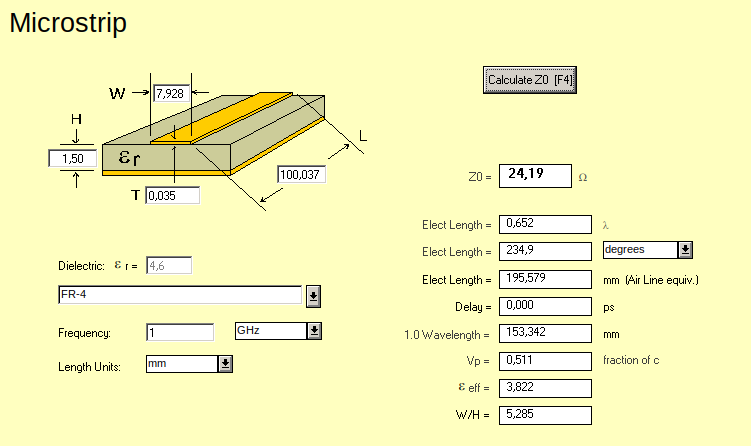
\includegraphics[scale=0.4]{../2carac/caract_large_bande/interface_AppCAD.png}
	\caption{Interface du logiciel AppCAD d'Agilent (exemple sur le calcul du verre epoxy fin)}
	\label{fig:interface_appcad}
\end{figure}




Le logiciel fournit également un paramètre appelé la permittivité diélectrique relative effective $\varepsilon_{reff}$, déjà évoqué dans le rapport. Il s'agit d'une grandeur utile pour considérer le mode de propagation comme un mode quasi-TEM. En effet, dans le cas réel la ligne micro-ruban est entourée d'un second milieu autre que le diélectrique, l'air. Il s'agit alors d'homogénéiser l'ensemble afin de passer d'un système à 2 milieux ($\varepsilon_r$ et $\varepsilon_0$) à 1 seul milieu ($\varepsilon_{reff}$). Un schéma de principe est précisé ci-dessous.

\begin{figure}[H]
	\centering
	\includegraphics[scale=0.4]{../2carac/caract_large_bande/image_1_non_homogene.png}
	\includegraphics[scale=0.4]{../2carac/caract_large_bande/image_2_homogene.png}
	\caption{Schéma du principe d'homogénéisation de la constante diélectrique}
	\label{fig:homogeneisation_epsilon_reff}
\end{figure}

Ce modèle simplifie grandement le mode de propagation puisqu'il est considéré comme non dispersif. Cependant ce modèle n'est valable que pour des fréquences faibles pour linéariser le mode dominant comme le montre le diagramme de dispersion (figure \ref{fig:diagramme_dispersion}). Au-delà de 10 GHz le mode quasi-TEM n'est plus valide et il est nécessaire de passer à un mode de propagation dispersif.\\
En remarque supplémentaire, l'approximation quasi-TEM est indispensable car celle-ci constitue la base de la formation de toutes les grandeurs et formules utilisées au cours de ce rapport. Par exemple, sans une telle approximation il est impossible de définir une impédance caractéristique $Z_C$ pour le milieu.

\begin{figure}[H]
	\centering
	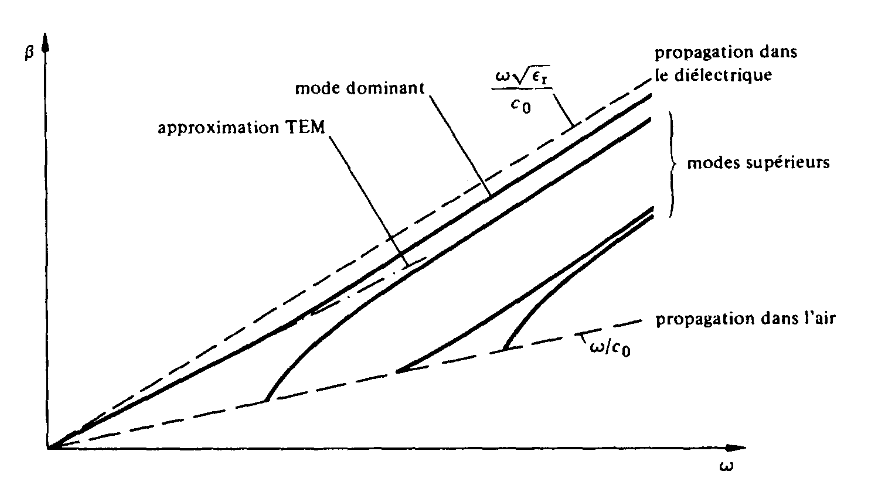
\includegraphics[scale=0.3]{../2carac/caract_large_bande/approx_QTEM.png}
	\caption{Diagramme de dispersion de la ligne micro-ruban}
	\label{fig:diagramme_dispersion}
\end{figure}

\newpage

\subsection{Caractérisation faible bande des lignes micro-rubans}
La partie précédente s'est chargée de détailler une première démarche pour caractériser une ligne micro-ruban. Elle s'appuie sur la correspondance entre un modèle théorique simulé sous ADS et des mesures pratiques. La mise en place d'une simulation nécessite d'avoir sous la main des outils logiciels complexes. Dans cette partie, une seconde méthode, plus simple, dite de "coin de table" va être présentée. Elle a l'avantage de faire appel uniquement à des calculs simples. En contrepartie le résultat obtenu n'est valable que sur une partie de la bande passante. Les équations utilisées se basent sur un modèle de substrat sans pertes où $tan( \delta)$ est négligé. Ainsi, seule la constante diélectrique $\varepsilon_r$ est obtenue avec cette méthode. \\
La mesure s'effectue comme pour la méthode précédente sur une ligne micro-ruban de longueur l, de hauteur h et largeur w connues comme sur la figure \ref{fig:modele_microstrip}. Nous prendrons l'exemple de la ligne de téflon large déjà caractérisée dont les données sont disponibles dans le tableau \ref{tab:geo_ligne}. Le coefficient de réflexion $S_{11}$ de cette ligne lorsqu’elle est chargée par 50$\Omega$ en sortie est le suivant :
\begin{figure}[H]
	\centering
	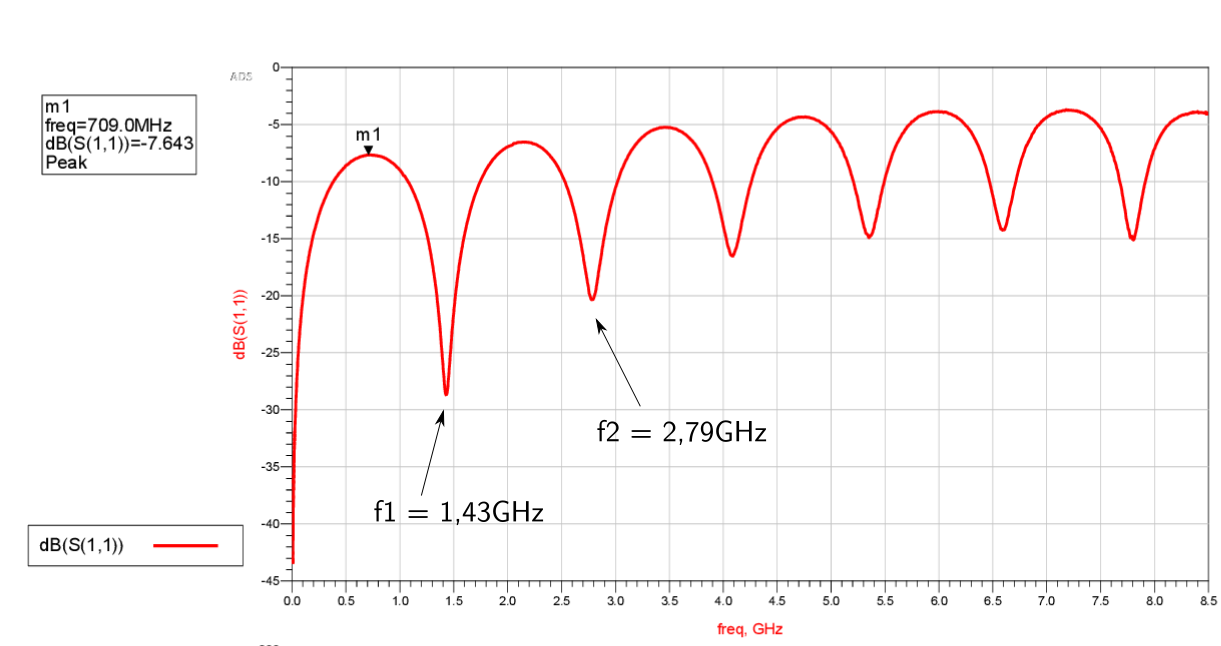
\includegraphics[width=0.7\linewidth]{../2carac/S11_ADS/teflonLarge_commente}
	\caption{Paramètre $S_{11}$ caractérisation faible bande teflon large}
	\label{fig:teflonlargecommente}
\end{figure}
La figure \ref{fig:teflonlargecommente} illustre le relevé du coefficient de réflexion sur une ligne teflon large. On observe une périodicité qui s'explique de la façon suivante. L'impédance $Z_c$ de la ligne ne vaut pas 50$\Omega$, mais aux fréquences multiples de $\lambda /2$ (fréquence de résonance), l'impédance vue en entrée est de 50$\Omega$ et le coefficient de réflexion est nul. Aux fréquences de résonances, dont les premières sont repérées sur la figure \ref{fig:teflonlargecommente}, on a l'égalité suivante donnant la vitesse V fonction de l'écart entre $F1$ et $F2$ et de la longueur L :  
\begin{equation}
V=2.L(F2-F1) 
\end{equation}
Application numérique avec L = 74,82mm, $F_1$ = 1,43GHz et $F_2$ = 2,79GHz :
\begin{equation}
V= 2*74,82*10^{-3}(2,79-1,43)10^9=203.10^6m.s^{-1}
\end{equation}
Nous avons également $\varepsilon_{reff}$ fonction de la célérité C et de la vitesse V :
\begin{equation}
\varepsilon_{reff} = \Big(\frac{C}{V}\Big)^2
\end{equation}
Application numérique avec C = $3.10^8m.s^{-1}$ et V = $203.10^6m.s^{-1}$ :
\begin{equation}
\varepsilon_{reff} = \Big(\frac{3.10^8}{203,5.10^6}\Big)^2=2,173 F.m^{-1}
\end{equation}
Et finalement, dans le cas d'une ligne micro-rubans, l'expression liant $\varepsilon_{reff}$ en fonction des paramètres de la lignes est la suivante :
\begin{equation}
	\varepsilon_{reff} = \frac{\varepsilon_r+1}{2}+\frac{\varepsilon_r-1}{2}\sqrt{1+\frac{10h}{w}}
\end{equation}
En expriment non pas $\varepsilon_{reff}$ mais $\varepsilon_{r}$ fonction des autres éléments on obtient : 
\begin{equation}
\varepsilon_{r} = \frac{2\varepsilon_{reff} + \sqrt{1 + \cfrac{10h}{w}} - 1}{1 + \sqrt{1 + \cfrac{10h}{w}}}
\end{equation}
Le résultat de l'application numérique avec h = 1,58mm, w = 7,87mm et L=74,83mm est donné par un script Octave pour limiter les erreurs de frappe et conserver des décimales. La constante diélectrique $\varepsilon_{r}$ du téflon large caractérisée sur la bande $[1,43;2,79]GHz$ est de 2,4881. La valeur obtenue est parfaitement cohérente avec les données du constructeur CIF qui donne une plage comprise entre 2,4 et 2,65. Cette seconde méthode pour caractériser la constante diélectrique des lignes micro-rubans offre de bons résultats et permet de gagner du temps dans le cas d'une étude large bande d'un substrat sans pertes.


\newpage

\section{Synthèse de filtre passe-bas Tchebychev en technologie micro-ruban}

\subsection{Choix des valeurs de composants}

L'objectif est de réaliser un filtre passe-bas dont le gabarit est donné à la figure \ref{fig:gabarit_PasseBas}. Le type de réponse souhaité est une réponse de Tchebychev.

\begin{figure}[H]
	\centering
	\includegraphics[width=0.5\linewidth]{ressources/gabarit_passe_bas}
	\caption{Gabarit filtre passe-bas équivalent}
	\label{fig:gabarit_PasseBas}
\end{figure}

Les valeurs numériques associées au gabarit sont les suivantes.
\begin{table}[H]
	\centering
	\begin{tabular}{|c|c|c|c|}
		\hline
		$A_{max}$& $A_{min}$ & $f_s$ & $f_c$ \\ \hline
		0.1	dB & 15,00 dB 		& 2 GHz	   & 3 GHz \\ \hline
	\end{tabular}
	\caption{Valeur numérique gabarit souhaité}
\end{table}
La conception d'un filtre hautes-fréquences débute par une synthèse classique avec des éléments passifs (condensateurs et bobines) comme il a été fait dans le module des moyennes fréquences du semestre 7. À partir du gabarit de la figure \ref{fig:gabarit_PasseBas}, l'équation ci-dessous permet d'obtenir l'ordre du filtre à concevoir.


\begin{equation}
	n \geq \cfrac{argch(\sqrt{\cfrac{\alpha_{min}-1}{\alpha_{max} -1}})}{argch(1/k)}
\end{equation}
On rappelle :
\begin{equation}
argch(x)=ln(x+\sqrt{x^2-1})
\end{equation}

Où :
\begin{itemize}
	\item n est l'ordre du filtre souhaité;
		\item k est la sélectivité égal à : 
	\begin{equation}
	k=\frac{f_s}{1,5f_s} = \frac{2}{3} \approx 0,67
	\end{equation}
	\item $\alpha_{min}$ est l'atténuation minimale (en linéaire) du signal dans la bande atténué égal à $10^{\frac{15}{10}} \approx 31,6$
	\item $\alpha_{max}$ est l'atténuation maximale (en linéaire) du signal dans la bande passante égal à $10^{\frac{0,1}{10}} \approx 1,02$
\end{itemize}

L'application nous donne $n \geq 4,5$ soit au minimum un ordre 5 pour respecter le gabarit souhaité. Le schéma passe-bas en impédance que nous allons utiliser est donné ci-dessous par la figure \ref{fig:gabarit_PB}.

\begin{figure}[H]
	\centering
	\begin{circuitikz}
		\draw (0,0)
		to[V,v=$U_e$] (0,2) % The voltage source
		to[L=$g_1$] (2,2)
		to[C=$g_2$] (2,0) % The resistor
		(2,2)to[L=$g_3$] (4,2)
		to[C=$g_2$] (4,0) % The resistor
		(4,2)to[L=$g_3$] (6,2)
		to [R=$r$] (6,0) 
		to[short] (0,0);
	\end{circuitikz}
	\caption{Schéma prototype d'un filtre passe-bas en impédance.}
\end{figure}

Avec :
\begin{itemize}
	
	\item les coefficients $g_k$, les valeurs normalisées des condensateurs et des bobines;
	\item r, la résistance de charge normalisée est égale à 1. Sa valeur dénormalisée est de $50\Omega$;
	\item $U_e$, le signal d'entrée ayant une résistance série normalisée égale à 1 et donc $50\Omega$ en dénormalisée.
\end{itemize}

Pour obtenir les valeurs de $g_k$ nous ne pouvons utiliser les tableaux donnés dans le polycopié d'électronique moyennes fréquences car ils ne sont valables uniquement pour des ondulations de 0.5 dB et 1 dB. Le gabarit impose une ondulation maximale de 0.1 dB dans la bande passante. Pour obtenir des coefficient $g_k$ qui permettent de respecter l'ondulation voulue, un script est réalisé sur Octave disponible en annexe. Le résultat obtenu est le suivant.

\begin{table}[H]
	\centering
	\begin{tabular}{|c|c|c|c|c|}
		\hline
		$g_1$ & $g_2$ & $g_3$ & $g_4$ & $g_5$\\
		\hline
		1.1468 & 1.3712 & 1.9750 & 1.3712 & 1.1468\\
		\hline
	\end{tabular}
	\caption{Valeurs des composants normalisées pour une ondulation de 0.1 dB}
	\label{tab:coefficient_g_k_passe_bas}
\end{table}
 
Pour trouver les valeurs réelles des composants il faut : pour les condensateurs, multiplier les $g_k$ pairs par un coefficient $C_{denom}$ et pour les bobines, multiplier les $g_k$ impairs par un coefficient $L_{denom}$. Les valeurs de ces coefficients sont données ci-dessous.

\begin{equation}
	C_{denom} = \frac{1}{2\pi f_s R}
	\qquad
	L_{denom} = \frac{R}{2\pi f_s}
\end{equation}

Le tableau ci-dessous donne les applications numériques pour les composants du filtre avec $f_s = 2GHz$ et $R = 50\Omega$.

\begin{table}[H]
	\centering
	\begin{tabular}{|c|c|c|c|c|}
		\hline
		$L_1$ & $C_2$ & $L_3$ & $C_4$ & $L_5$\\
		\hline
		4.56 nH & 2.18 pF & 7.86 nH & 2.18 pF & 4.56 nH\\
		\hline
	\end{tabular}
	\caption{Valeurs réelles des composants du filtre passe-bas.}
	\label{tab:valeurs_composant_passe_bas}
\end{table}

Pour vérifier et valider les valeurs de composants du filtre, le logiciel ADS est utilisé. Le schéma simulé est celui de la figure \ref{fig:schema_distribue_ameliore_passe_bas_ads}. 

\begin{figure}[H]
	\centering
	\includegraphics[width=9cm]{photo/passe_bas_vic/schema_localise_passe_bas_ads.png}
	\caption{Schéma d'un filtre passe-bas avec des éléments localisés}
	\label{fig:schema_localise_passe_bas_ads}
\end{figure}

On note la présence de deux blocs S-PARAMETERS. Le premier permet une simulation sur la bande de fréquence $[0; 10\ GHz]$ pour observer le comportement général du filtre. Le second permet une simulation sur la bande $[0; 2\ GHz]$ pour avoir un zoom sur la bande passante et analyser l'ondulation en bande passante. La figure \ref{fig:simu_passe_bas_localise_global} montre le résultat de ces simulations.

\begin{figure}[H]
	\centering
	\begin{subfigure}[b]{0.49\textwidth}
		\includegraphics[width=\textwidth]{photo/passe_bas_vic/simu_passe_bas_localise.PNG}
		\caption{Sans zoom}
		\label{fig:simu_passe_bas_localise}
	\end{subfigure}
	\begin{subfigure}[b]{0.49\textwidth}
		\includegraphics[width=\textwidth]{photo/passe_bas_vic/simu_zoom_passe_bas_localise.PNG}
		\caption{Avec zoom sur la bande passante}
		\label{fig:simu_zoom_passe_bas_localise}
	\end{subfigure}
	\caption{Simulation du module de S21 en dB d'un filtre de tchebychef avec des éléments localisés}
	\label{fig:simu_passe_bas_localise_global}
\end{figure}

D'une manière globale on a bien un comportement de type basse-bas. L'ondulation en bande passante sur la figure \ref{fig:simu_zoom_passe_bas_localise} est comprise entre 0 et 0,1 dB comme souhaité par le cahier des charges. Au niveau des fréquences caractéristiques il faut observer que l'ondulation en bande passante est correctement conservée jusqu'à 2 GHz (fréquence de coupure nommée fs dans le gabarit de la figure \ref{fig:gabarit_PasseBas}). Au delà de 3 GHz (fréquence nommée fc sur la figure \ref{fig:gabarit_PasseBas}) l'atténuation du filtre est supérieure à 19 dB ce qui est conforme aux 15 dB d'atténuation minimum désiré par le cahier des charges. Les résultats observés à la figure \ref{fig:simu_passe_bas_localise_global} permettent donc de valider les valeurs des composants (condensateurs et bobines) au regard du cahier des charges. \\


La prochaine étape est de choisir une technologie pour implémenter ce filtre. C'est là que la subtilité des hautes-fréquences intervient. Le choix que l'on aurait fait en basse ou moyenne fréquence de prendre une technologie localisée (composants traversant et CMS)\footnote{Cette technologie est dite localisée car elle fait référence aux composants qui voient leurs tailles physiques grandes ou proches de la longueur d'onde des signaux qu'ils traitent.} serait faux. La principale raison est la prise en compte des effets inductifs qui était négligeable en basse et en moyenne fréquence va maintenant entraîner des effets parasites indésirables. La technologie proposée dans le cours est dite distribuée. Ce terme vient du fait que la longueur d'onde des signaux mises en jeu est proche de la taille des éléments physiques qui vont remplacer les capacités et les bobines voulues. Chaque éléments discrets (bobine et capacité) vont être remplacés par une ligne micro-ruban. Une ligne micro-ruban est une ligne de propagation qui peut avoir des effets capacitifs ou inductifs selon son dimensionnement. 

\subsection{La technologie micro ruban}
\subsubsection{Les lignes de transmission inductives}


Dans cette partie on cherche à remplacer les inductances séries du filtre par des lignes de transmission qui apportent le même effet capacitif. La figure \ref{fig:probleme_ligne_inductive} illustre les deux schémas qui seront utilisés.


\begin{figure}[H]
	\centering
	\begin{subfigure}[b]{0.3\textwidth}
		\begin{circuitikz}
			\draw (0,2)
			to [short,*-](0,2)
			node[above]{$Z_{vue}$}
			to[TL=$Z_c$\texttt{,} $l$] (2,2)
			to [generic=$Z_0$] (2,0) node[ground]{};
		\end{circuitikz}
	\end{subfigure}
	\begin{subfigure}[b]{0.3\textwidth}
		\begin{circuitikz}
			\draw (0,2)
			to [short,*-](0,2)
			node[above]{$Z_{vue'}$}
			to[L=$L$] (2,2)
			to [generic=$Z_0$] (2,0) node[ground]{};
		\end{circuitikz}
	\end{subfigure}
	\caption{Schéma d'une ligne de transmission apparentée à une inductance}
	\label{fig:probleme_ligne_inductive}
\end{figure}

On précise que $Z_c$ est l'impédance caractéristique de la ligne de transmission, $l$ est la longueur de la ligne, $L$ la valeur de l'inductance équivalente et $Z_0$ la charge. L'impédance vue en entrée de la ligne de transmission est donnée par la formule :

\begin{equation}
	Z_{vue} = Z_c\ \frac{Z_0 + j Z_c tan(\beta l)}{Z_c + j Z_0 tan(\beta l)}
\end{equation}

Dans le cas où l'on choisit une ligne de transmission avec une impédance caractéristique très supérieure à l'impédance de charge on a $Z_c>>Z_0$ et donc :

\begin{equation}
	Z_{vue} = Z_0 + j Z_c tan(\beta l)
\end{equation}

L'impédance vue en entrée du montage avec la bobine idéale L est donnée par 

\begin{equation}
	Z_{vue'} = Z_0 + j 2\pi f L 
	\label{eq:ZvueL1}
\end{equation}

On a ici une évolution de l'impédance $Z_{vue'}$ proportionnelle à la fréquence. Dans le cas de la ligne de transmission on rappelle que la constante de phase $beta$ est reliée à la fréquence par la formule :

\begin{equation}
	\beta = \frac{2 \pi f}{v_\phi}
\end{equation}

Où $f$ est la fréquence en Hz et $v_\phi$ la vitesse de l'onde électromagnétique dans la ligne en m/s. On sait aussi que pour de petites variations de x autour de 0, le développement limité de $tan(x)$ est égal à $x$ soit $tan(x)=x$ . Dans ces conditions on se trouve également avec une relation de proportionnalité entre $Z_{vue}$ et la fréquence :

\begin{equation}
	Z_{vue} = Z_0 + jZ_c\frac{2 \pi f}{v_\phi} l
	\label{eq:ZvueL2}
\end{equation}

Il nous est maintenant possible d'assimiler les équations \ref{eq:ZvueL1} et \ref{eq:ZvueL2} on obtient :

\begin{equation}
	Z_0 + j 2\pi f L = Z_0 + jZ_c\frac{2 \pi f}{v_\phi} l
\end{equation}

On isole l'inductance $L$.

\begin{equation}
	L = \frac{Z_c l}{v_\phi}
	\label{eq:resultat_L}
\end{equation}

On a ici l'expression d'une inductance en fonction des paramètres d'une ligne de transmission à savoir, son impédance $Z_c$ et de sa longueur $l$. 

\subsubsection{Les lignes de transmission capacitives}

Dans cette partie on cherche à remplacer les condensateurs parallèles du filtre par des lignes de transmission séries qui apportent le même effet capacitif. La figure \ref{fig:probleme_ligne_capacitive} illustre les deux schémas que nous utiliserons pour la démonstration de ce passage d'un condensateur à une ligne de transmission.

\begin{figure}[H]
	\centering
	\begin{subfigure}[b]{0.3\textwidth}
		\begin{circuitikz}
			\draw (0,2)
			to [short,*-](0,2)
			node[above]{$Z_{vue}$}
			to[TL=$Z_c$\texttt{,} $l$] (2,2)
			to [generic=$Z_0$] (2,0) node[ground]{};
		\end{circuitikz}
	\end{subfigure}
	\begin{subfigure}[b]{0.3\textwidth}
		\begin{circuitikz}
			\draw (0,2)
			to [short,*-](0,2)
			node[above]{$Z_{vue'}$}
			to [short](2,2)
			(2,2)to[C=$C$] (2,0)
			(2,0)node[ground]{}
			(2,2) to [short](4,2)
			(4,2)to [generic=$Z_0$] (4,0) node[ground]{};
		\end{circuitikz}
	\end{subfigure}
	\caption{Schéma d'une ligne de transmission apparentée à un condensateur}
	\label{fig:probleme_ligne_capacitive}
\end{figure}

Comme pour la partie précédente, on précise que $Z_c$ est l’impédance caractéristique de la ligne de transmission, $l$ est la longueur de la
ligne, $C$ la valeur de la capacité équivalente et $Z_0$ la charge. L’impédance vue en entrée de la ligne de transmission
est donnée par la formule :


\begin{equation}
	Z_{vue} = Z_c\ \frac{Z_0 + j Z_c tan(\beta l)}{Z_c + j Z_0 tan(\beta l)}
\end{equation}

Dans le cas où l'on choisit une ligne de transmission avec une impédance caractéristique très inférieure à l'impédance de charge on a $Z_c<<Z_0$ et donc :

\begin{equation}
	Z_{vue} = \frac{Z_c Z_0}{2_c + j Z_0 tan(\beta l)}
\end{equation}

On en déduit que l'admittance vue en entrée de la ligne de transmission est égale à :

\begin{equation}
	Y_{vue} = \frac{1}{Z_{vue}} = \frac{1}{Z_0} + \frac{j tan(\beta l)}{Z_c}
\end{equation}

Du côté de l'impédance vue en entrée du montage avec le condensateur C on a :

\begin{equation}
	Z_{vue'} = \frac{Z_0}{1 + j C Z_0 2 \pi f}
\end{equation}


Et donc une admittance $Y_{vue'}$ :

\begin{equation}
	Y_{vue'} =  \frac{1}{Z_{vue'}} = \frac{1}{Z_0} + j C 2 \pi f
	\label{eq:YvueC1}
\end{equation}


On a ici une évolution de l'admittance $Y_{vue'}$ proportionnelle à la fréquence. Dans le cas de la ligne de transmission on rappelle que la constante de phase $beta$ est reliée à la fréquence par la formule :

\begin{equation}
	\beta = \frac{2 \pi f}{v_\phi}
\end{equation}


Où $f$ est la fréquence en Hz et $v_\phi$ la vitesse de l'onde électromagnétique dans la ligne en m/s. On sait aussi que pour de petites variations de x autour de 0, le développement limité de $tan(x)$ est égal à $x$ soit $tan(x)=x$. Dans ces conditions on se trouve également avec une relation de proportionnalité entre $Y_{vue}$ et la fréquence :

\begin{equation}
	Y_{vue} = \frac{1}{Z_{vue}} = \frac{1}{Z_0} + \frac{j 2\pi f}{v_\phi Z_c} l
	\label{eq:YvueC2}
\end{equation}

Il nous est maintenant possible d'assimiler les équations \ref{eq:YvueC1} et \ref{eq:YvueC2} on obtient :

\begin{equation}
	\frac{1}{Z_0} + j C 2 \pi f = \frac{1}{Z_0} + \frac{j 2\pi f}{v_\phi Z_c} l
\end{equation}

On isole la capacité $C$.

\begin{equation}
	C = \frac{l}{Z_c v_\phi}
	\label{eq:resultat_C}
\end{equation}

On a ici une expression d'une capacité en fonction des paramètre d'une ligne de transmission à savoir, son impédance $Z_c$ et de sa longueur $l$. 


\subsubsection{Limites de validité}

Comme nous l'avons vu dans les parties précédentes, des lignes de transmission peuvent s'apparenter à des effets capacitifs ou inductifs sous certaines conditions. Ces conditions sont aux nombres de deux. La première est sur l'impédance de la ligne de transmission $Z_c$ tandis que la deuxième est liée au terme $\beta l$ contenue dans l'expression de l'impédance ramenée.\\
%La condition du $Z_c$ est lié aux contraintes dépend de la largeur des pistes et donc de des procédés de fabrication. Cette condition sera abordé dans la partie suivante sur le passage des composants discret à des lignes de transmission. Il nous reste donc la

\textbf{Condition du $Z_c$\\}

Nous allons voir que la condition sur $Z_c$ est directement liée à la largeur des lignes de transmission.

Dans le cas où l'on cherche à \underline{apparenter une bobine série avec une charge} à une ligne de transmission série avec une charge, son impédance caractéristique doit être très supérieure à $Z_0$ soit $Z_c >> Z_0$. Dans ces conditions l'impédance $Z_c$ s'écrit :

\begin{equation}
	Z_c = \frac{119,9}{\sqrt{2(\epsilon_r + 1)}} \left[ ln\left(4\frac{h}{w} + \sqrt{16\left(\frac{h}{w}\right)^2 + 2}\right) - \frac{1}{2}\left(\frac{\epsilon_r - 1}{\epsilon_r + 1}\right) \left(ln\frac{\pi}{2} + \frac{1}{\epsilon_r}ln\frac{4}{\pi}\right) \right]
	\label{eq:Z_c_bobine}
\end{equation}

Où $\epsilon_r$ est la permittivité relative du substrat en F/m, $h$ est l'épaisseur de cuivre en mm et $w$ la largeur de la piste de cuivre en mm. La permittivité relative est donnée par le constructeur où alors elle peut être trouvée de manière expérimentale comme on a pu le faire dans les premières séances de TP (cf partie sur la caractérisation). Dans notre cas l'épaisseur h a une valeur standard de 1,58 mm. La largeur $w$ quant à elle, dépend des procédés de fabrication. Au vu de l'expression de $Z_c$, sachant $Z_0=50 \Omega$ où w de 4,8 mm (donnée dans le sujet du TP) et sachant également l'expression de $Z_c$ ainsi que $Z_c >> Z_0$, on en déduit qu'il faut $w << 4,8$ mm. Les contraintes technologiques nous permettent de faire des pistes de cuivre ayant \underline{une largeur $w$ de 0,5 mm}.\\

Dans le cas où l'on cherche à \underline{apparenter un condensateur parallèle avec une charge} à une ligne de transmission série avec une charge, son impédance caractéristique doit être très inférieure à $Z_0$ soit $Z_c << Z_0$. Dans ces conditions l'impédance $Z_c$ s'écrit :

\begin{equation}
	Z_c= \frac{119,9\pi}{2\sqrt{\epsilon_r}}\left[\frac{w}{2h} + \frac{ln4}{\pi} + \frac{ln(e\pi^2 / 16)}{2\pi}\left(\frac{\epsilon_r + 1}{\epsilon_r}\right) + \frac{\epsilon_r + 1}{2\pi \epsilon_r} \left( ln\frac{\pi e}{2} +  ln\left(\frac{w}{2h} + 0,94 \right) \right)  \right]^{-1}
	\label{eq:Z_c_condo}
\end{equation}


Où $\epsilon_r$ est la permittivité relative du substrat en F/m, $h$ est l'épaisseur de cuivre en mm et $w$ la largeur de la piste de cuivre en mm. La permittivité relative est donnée par le constructeur où alors elle peut être trouvée de manière expérimentale comme on a pu le faire dans les premières séances de TP (cf partie sur la caractérisation). Dans notre cas l'épaisseur h a une valeur standard de 1,58 mm. La largeur $w$ quant à elle, dépend des procédés de fabrication. Au vu de l'expression de $Z_c$, sachant $Z_0=50 \Omega$ où w de 4,8 mm (donnée dans le sujet du TP) et sachant également l'expression de $Z_c$ ainsi que $Z_c << Z_0$, on en déduit qu'il faut $w >> 4,8$ mm. Les contraintes technologiques nous permettent de faire des pistes de cuivre ayant \underline{une largeur $w$ de 10 mm}.\\


\textbf{Condition du $\beta l$\\}

Lors de la présentation de la technologie micro ruban nous avons linéarisé l'expression $tan(\beta l)$ en disant que $tan(\beta l)=\beta l$ pour de petites variations de $\beta l$. Étudions maintenant ces conditions plus en détail. Pour ce faire on commence par tracer sur la figure \ref{fig:tan_x} la fonction $y = tan(x)$

\begin{figure}[H]
	\centering
	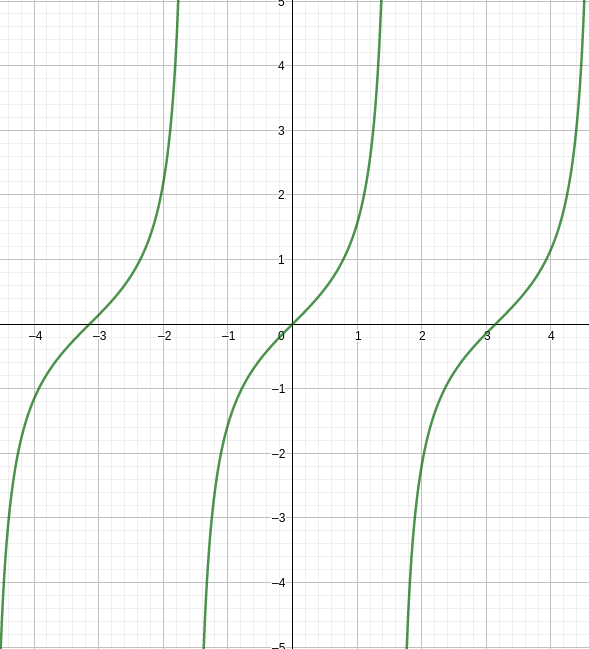
\includegraphics[width=6cm]{photo/tan_x.png}
	\caption{Tracé de la fonction tangente de x}
	\label{fig:tan_x}
\end{figure}

La fonction $tan(x)$ n'est définie que sur l'intervalle $[-\frac{\pi}{2}; \frac{\pi}{2}]$. D'après le développement limité de Taylor et de manière graphique on observe bien que plus x est proche de 0 et plus l'expression $tan(x) = x$ est vraie. On en déduit que pour linéariser l'expression il faut $x << \frac{\pi}{2}$. Dans notre application $tan(x) = tan(\beta l)$ donc $x = \beta l$. On rappelle que $\beta$ peut s'écrire :

\begin{equation}
	\beta = \frac{2 \pi}{\lambda}
\end{equation}

Où $f$ est la fréquence de l'onde électromagnétique en Hz et $v_\phi$ la vitesse de propagation en m/s. D'après les dire précédent pour linéariser la tangente $x << \frac{\pi}{2}$ soit $\beta l << \frac{\pi}{2}$ ce qui nous donne la condition sur $l$ :

\begin{equation}
	l << \frac{\lambda}{4}
\end{equation}

Cette condition nous indique que la longueur de la ligne de transmission $l$ doit être très inférieure à $\frac{\lambda}{4}$ pour que les lignes de transmissions puissent s'apparenter correctement à des bobines ou à des condensateurs.


\subsection{Passage des composants discrets à des lignes de transmission}

\subsubsection{Introduction et rappel}

Dans cette partie on cherche à remplacer les éléments localisés du filtre de la figure \ref{fig:schema_localise_passe_bas_ads} par des lignes de transmission. On part des expressions \ref{eq:resultat_L} et \ref{eq:resultat_C} que l'on tourne pour obtenir une expression de la longueur des lignes de transmission. On appellera $l_C$ la longueur des lignes qui vont s'apparenter à des condensateurs et $l_L$ la longueur des lignes qui vont s'apparenter à des bobines.

\begin{equation}
	l_L = \frac{L v_\phi}{Z_c}
	\qquad
	l_C = C Z_c v_\phi
	\label{eq:expression_l}
\end{equation}

Avec $Z_c$, l'impédance caractéristique de la ligne de transmission (ATTENTION : la valeur est différente pour les bobines et les condensateurs) en Ohms, $l_C$ et $l_L$ en m, $L$ en H, $C$ en F et $v_\phi$ en m/s dont l'expression est donnée par :

\begin{equation}
	v_\phi = \frac{3.10^8}{\sqrt{\epsilon_{reff}}}
\end{equation}

Où $\epsilon_{reff}$ est la permittivité relative effective du matériau sans unité et s'exprime par : 

\begin{equation}
	\epsilon_{reff} = \frac{\epsilon_r + 1}{2} + \frac{\epsilon_r - 1}{2}\left(1 + \frac{10h}{w}\right)^{-1/2}
	\label{eq:espilon_reff}
\end{equation}


\subsubsection{Transformation des éléments localisés en éléments distribués}

L'objectif ici est de déterminer les paramètres des lignes de transmissions qui vont remplacer les bobines et les condensateurs. Ces paramètres sont : la permittivité relative du substrat, l'impédance caractéristique de la ligne, la hauteur de cuivre, sa largeur et sa longueur.\\
On commence par le \underline{remplacement de toutes les bobines}. On fait le choix de détailler les calculs \underline{pour un substrat en teflon} de permittivité relative 2,624 obtenue à partir des plaques de teflon large lors de la partie sur la caractérisation. On se base sur une hauteur de cuivre $h$ standard de 1,580 mm et une largeur de piste $w$ de 0,500 mm tel que montré dans la partie sur les limites de validités. A partir de tous ces éléments et des équations \ref{eq:espilon_reff} et \ref{eq:Z_c_bobine} on trouve :

\begin{equation}
	\epsilon_{reff} = 1,954
	\qquad
	Z_c = 138,090 \Omega
\end{equation}

Il ne nous reste plus qu'à calculer les longueurs des lignes de transmissions qui vont remplacer les bobines. Pour cela on utilise l'expression de $l_L$ de la formule \ref{eq:expression_l}. Le tableau ci-dessous récapitule les longueurs obtenues en fonction des valeurs des bobines.


\begin{table}[H]
	\centering
	\begin{tabular}{|c|c|c|}
		\hline
		$L$ & 4,560 nH & 7,850 nH \\
		\hline
		$l_L$ & 7,086 mm & 12,200 mm\\
		\hline
	\end{tabular}
	\caption{Longueurs des lignes de transmission qui remplacent les bobines pour le substrat en teflon}
	\label{tab:longueur_ligne_bobine_passe_bas}
\end{table}


On s'attaque maintenant au \underline{remplacement des condensateurs}. On fait les mêmes choix de valeurs pour la permittivité relative (2,624) et pour la hauteur de cuivre (1,580 mm). Pour la largeur de cuivre, conformément à la partie sur les limites de validité on prendra une largeur de 10 mm. Pour le calcul de $\epsilon_{reff}$ on utilise toujours l'équation \ref{eq:espilon_reff} tandis que pour $Z_c$ on utilise maintenant la formule \ref{eq:Z_c_condo} ce qui donne :

\begin{equation}
	\epsilon_{reff} = 2,318\
	\qquad
	Z_c = 26,965 \Omega
\end{equation}

Il ne nous reste plus qu'à calculer les longueurs des lignes de transmissions qui vont remplacer les bobines. Pour cela on utilise l'expression de $l_C$ de la formule \ref{eq:expression_l}. Le filtre contient une seule valeur de capacité : 2,18 pF. Cela fait que nous avons qu'une seule longueur à calculer :

\begin{equation}
	l_C = \frac{2,18.10^{-12} * 26,965 * 3.10^8}{\sqrt{2,318}} = 11,584 mm
\end{equation}



\subsubsection{Simulation sur le substrat de teflon}

Pour vérifier nos valeurs obtenues on passe sur le logiciel de simulation ADS. Le schéma réalisé est disponible à la figure \ref{fig:schema_distribue_passe_bas_ads}. Il est composé de cinq éléments mis en série. Aux extrémités on trouve deux terminaux (ou charge) $50\Omega$. Les éléments mis en série sont des lignes de transmission basées avec une largeur W, une longueur L et un substrat teflonLarge. Les deux premiers paramètres sont selon les résultats obtenus dans les parties précédentes. Pour le substrat on utilise un bloc MSub que l'on appellera teflonLarge. Il contient toutes les informations concernant le substrat sur lequel on souhaite simuler notre filtre. On y trouve par exemple la permittivité relative du matériau, la hauteur du cuivre voulue ou encore les pertes liées à $tan(\delta)$.

\begin{figure}[H]
	\centering
	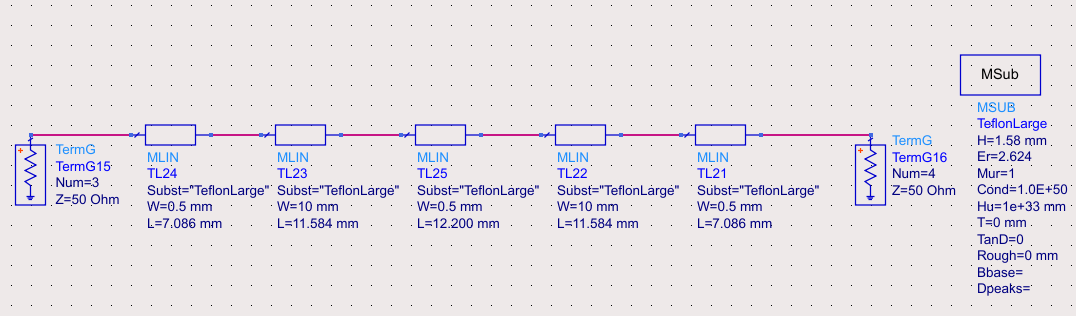
\includegraphics[width=15cm]{photo/passe_bas_vic/schema_distribue_passe_bas_ads.png}
	\caption{Schéma d'un filtre passe-bas de tchebychef en technologie micro ruban}
	\label{fig:schema_distribue_passe_bas_ads}
\end{figure}

Pour valider le comportement du filtre on affiche le coefficient de transmission S21. La figure \ref{fig:simu_passe_bas_distribue} contient le résultat de la simulation sur deux intervalles de fréquences. A gauche, on observe le comportement général du filtre sans avoir de détails sur la bande passante tandis qu'à droite on y a un zoom.

\begin{figure}[H]
	\centering
	\begin{subfigure}[b]{0.49\textwidth}
		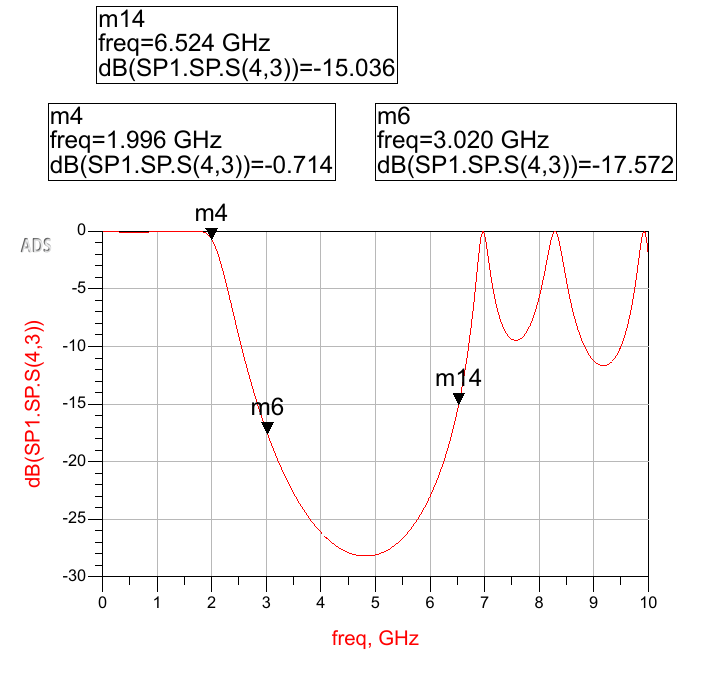
\includegraphics[width=\textwidth]{photo/passe_bas_vic/simu_passe_bas_distribue.PNG}
		\caption{Sans zoom}
		\label{fig:simu_passe_bas_distribueG}
	\end{subfigure}
	\begin{subfigure}[b]{0.49\textwidth}
		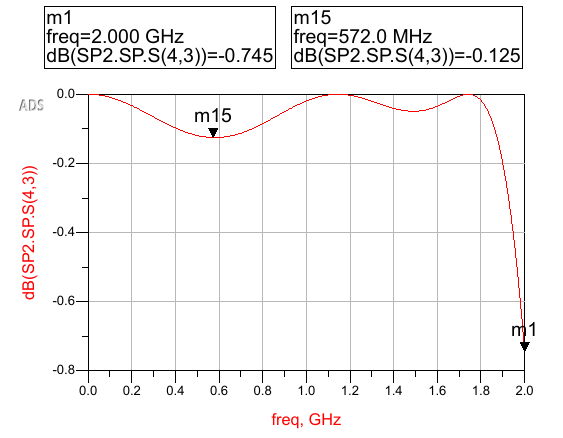
\includegraphics[width=\textwidth]{photo/passe_bas_vic/simu_zoom_passe_bas_distribue.PNG}
		\caption{Avec zoom sur la bande passante}
		\label{fig:simu_zoom_passe_bas_distribue}
	\end{subfigure}
	\caption{Simulation du module de S21 en dB d'un filtre de tchebychef en technologie micro ruban}
	\label{fig:simu_passe_bas_distribue}
\end{figure}


Sur la figure \ref{fig:simu_passe_bas_distribueG} on observe le comportement d'un filtre passe-bas avec une fréquence de coupure à environ 2 GHz. Du côté de la bande passante l'atténuation va jusqu'à 0,745 dB (pour 2 GHz) ce qui est supérieur aux 0,1 dB voulues par le cahier des charges. Au niveau de la bande atténuée, l'atténuation commence à 17 dB (à 3 GHz) ce qui respecte le gabarit (qui imposait 15 dB) jusqu'à la fréquence approximative de 6,5 GHz uniquement. A partir de cette fréquence (et depuis 4,5 GHz environ) le coefficient de transmission remonte puis fait des "va et vient" à 0 dB sous la forme de lobes.\\


La justification de ces lobes vient de l'expression de l'impédance ramenée et particulièrement du terme $tan(\beta l)$. Dans la partie sur la technologie micro ruban il a été dit que pour linéariser la tangente il faut $l << \frac{\lambda}{4}$. On rappelle le lien entre la longueur d'onde et la fréquence :

\begin{equation}
	\lambda = \frac{v_\phi}{f}
\end{equation}

Avec $\lambda$ la longueur d'onde en m, $f$, la fréquence de l'onde électromagnétique en Hz et $v_\phi$ la vitesse de propagation de l'onde électromagnétique. Dans cette formule on observe que la longueur d'onde diminue lorsque la fréquence augmente. Il est logique de dire que $\lambda$ sera inférieure aux longueurs des lignes de transmission qui s'apparentent aux bobines ou aux condensateurs. Prenons par exemple la bobine L2 de la figure \ref{fig:schema_localise_passe_bas_ads} qui est remplacé une ligne de transmission avec une longueur de 12,200 mm. Au premier creux de la figure \ref{fig:simu_passe_bas_distribueG}, la fréquence est à 4,5 GHz ce qui donne une longueur d'onde de 47,690 mm. La condition sur la longueur de la ligne qui implique que $l << \frac{\lambda}{4}$ n'est plus respectée. On se retrouve avec $l > \frac{\lambda}{4}$ car $12,208 mm\ >\ 11,922 mm$. Plus on augmente la fréquence et moins la condition que l'on avait posé au départ est vraie. Les croissances et décroissances du coefficient de transmission S21 peuvent également être justifier avec la figure \ref{fig:tan_x} qui montre que la composante $tan(x)$ (ou $tan(\beta l)$) est définie uniquement sur l'intervalle $[-\frac{\pi}{2}: \frac{\pi}{2}]$ puis se répète avec une période $\pi$. Quand x devient supérieure à $\frac{\pi}{2}$ la tangente devient négative jusqu'à $\pi$ puis redevient positive jusqu'à $\frac{3 \pi}{2}$ etc. Ce comportement fait que l'impédance ramené de la ligne de transmission va évoluer au rythme de la tangente et donc de façon périodique, avoir de brusques changements.\\


Du côté de la bande passante, il juste de se demander pourquoi on ne respecte par le gabarit. Comme pour les lobes cela est dû à la composante $tan(\beta l)$ que l'on a linéarisée. Le problème est que $\beta l$ est toujours en dessous de la valeur de $tan(\beta l)$ ce qui se traduit par une chute de la fréquence de coupure. Lorsque l'on fait $tan(\beta l) \approx \beta l$, l'ordre de grandeur de l'erreur de l'approximation est de 20\%.\\

Une autre chose intéressante a noter est au niveau des paramètres du substrat. Dans la simulation présentée ci-dessus les pertes liées au substrat traduites par $tan(\delta)$ étaient nulles ce qui n'est pas le cas dans la réalité. Mettons $tan(\delta) = 0,1$ pour observer l'impact sur la réponse en fréquence du filtre.

\begin{figure}[H]
	\centering
	\begin{subfigure}[b]{0.49\textwidth}
		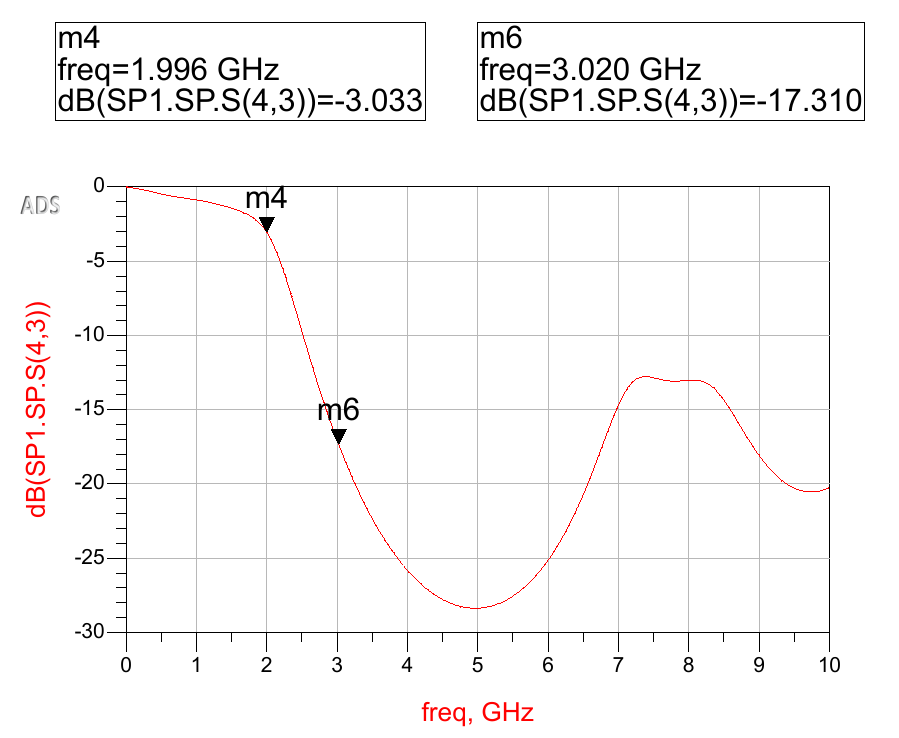
\includegraphics[width=\textwidth]{photo/passe_bas_vic/simu_passe_bas_distribue_substrat_avec_perte.PNG}
		\caption{Sans zoom}
		\label{fig:simu_passe_bas_distribue_substrat_avec_perteG}
	\end{subfigure}
	\begin{subfigure}[b]{0.49\textwidth}
		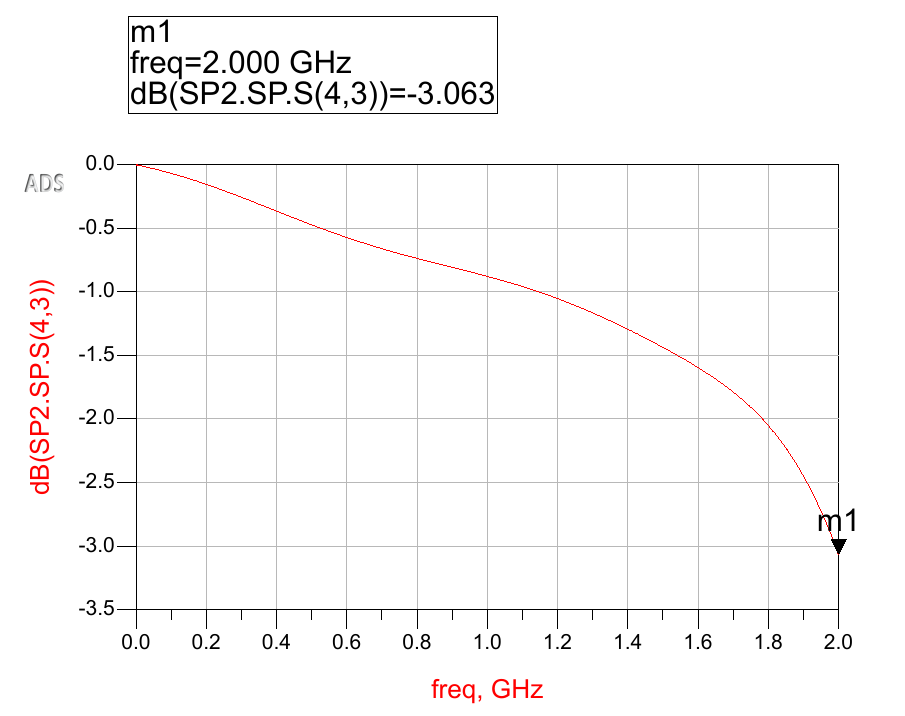
\includegraphics[width=\textwidth]{photo/passe_bas_vic/simu_zoom_passe_bas_distribue_substrat_avec_perte.PNG}
		\caption{Avec zoom sur la bande passante}
		\label{fig:simu_zoom_passe_bas_distribue_substrat_avec_perte}
	\end{subfigure}
	\caption{Simulation du module de S21 en dB d'un filtre de tchebychef en technologie micro ruban avec des pertes liées au substrat}
	\label{fig:simu_passe_bas_distribue_substrat_avec_perte}
\end{figure}

En comparaison avec la figure \ref{fig:simu_passe_bas_distribue}, on note que le coefficient de transmission S21 ne remonte pas à 0. En effet, au lieu d'être plus ou moins centré sur 0 dB, l'atténuation sur la figure \ref{fig:simu_zoom_passe_bas_distribue_substrat_avec_perte}, semble suivre une droite à pente négative. Au niveau de 7GHz, alors que l'atténuation allait jusqu'à 0 dB, là, elle ne remonte pas au delà de -12 dB. On note que cela est toujours inférieure à la droite imaginaire que l'on pourrait tracer à partir de la réponse dans la bande passante.


\subsubsection{Amélioration de la réponse fréquentielle}

On a relevé sur la figure \ref{fig:simu_passe_bas_distribue} que le comportement passe-bas n'est pas respecté dans la bande passante mais qu'il l'est sur la bande atténuée pour des fréquences comprises entre 3 GHz et 6,5 GHz. Nous allons voir qu'il est possible d'augmenter la plage de fréquence de cette bande atténuée en ajoutant un stub avec une distance et une fréquence de caractéristique bien choisie. Nous placerons ce stub à l'une des extrémités du filtre. \\

Pour ne pas amener un court-circuit directement dans les basses fréquences nous faisons le choix de prendre un stub à circuit ouvert. L'idée est d'apporter un 0 de transmission (un court circuit) à une fréquence donnée. De cette façon, on serait certain qu'à cette fréquence nous n'avons pas de transmission. Cette non transmission se traduit par un coefficient S21 égal à moins l'infini. Pour apporter un 0 de transmission avec un stub ouvert il nous faut choisir une longueur de stub égal à $\frac{\lambda}{4}$. Du côté de la fréquence caractéristique du stub, nous faisons le choix de la mettre à 7 GHz où le coefficient S21 est retourné à 0 dB. La figure \ref{fig:schema_distribue_ameliore_passe_bas_ads} montre le nouveau schéma du filtre.

\begin{figure}[H]
	\centering
	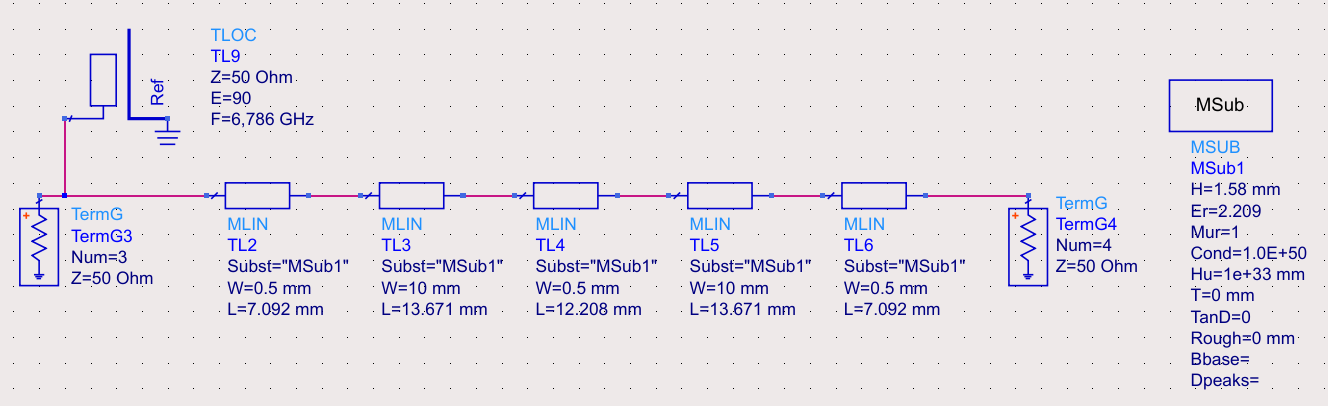
\includegraphics[width=15cm]{photo/passe_bas_vic/schema_distribue_ameliore_passe_bas_ads.png}
	\caption{Schéma d'un filtre passe-bas de tchebychev amélioré en technologie micro ruban.}
	\label{fig:schema_distribue_ameliore_passe_bas_ads}
\end{figure}

On note que la longueur du stub est liée au paramètre E, la longueur électrique en degrés qui est égale au produit : $\beta l$. Sachant que l'on souhaite une longueur de stub égale à $\frac{\lambda}{4}$ pour une fréquence de 7 GHz, nous avons mis une valeur de 90° pour le paramètre E. La figure \ref{fig:simu_passe_bas_distribue_ameliore} est le résultat de la simulation.

\begin{figure}[H]
	\centering
	\begin{subfigure}[b]{0.49\textwidth}
		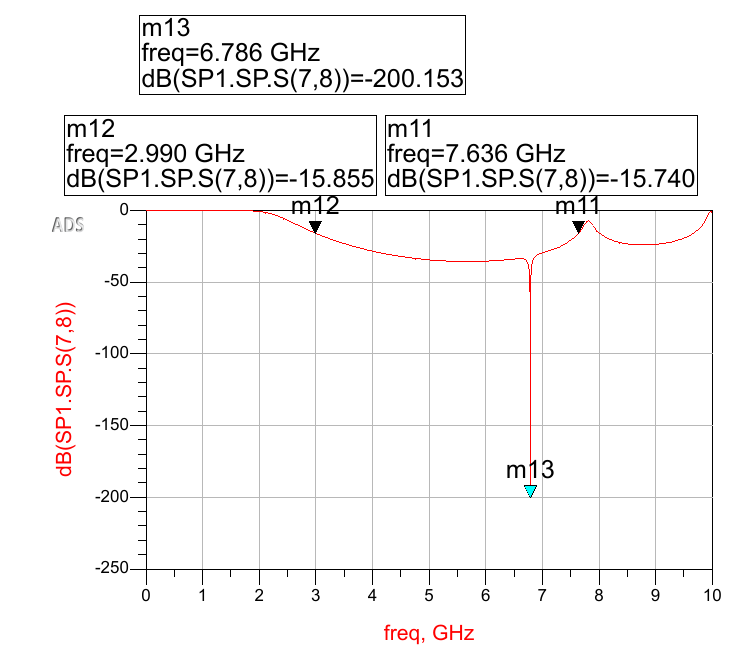
\includegraphics[width=\textwidth]{photo/passe_bas_vic/simu_passe_bas_distribue_ameliore.PNG}
		\caption{Sans zoom}
		\label{fig:simu_passe_bas_distribue_amelioreG}
	\end{subfigure}
	\begin{subfigure}[b]{0.49\textwidth}
		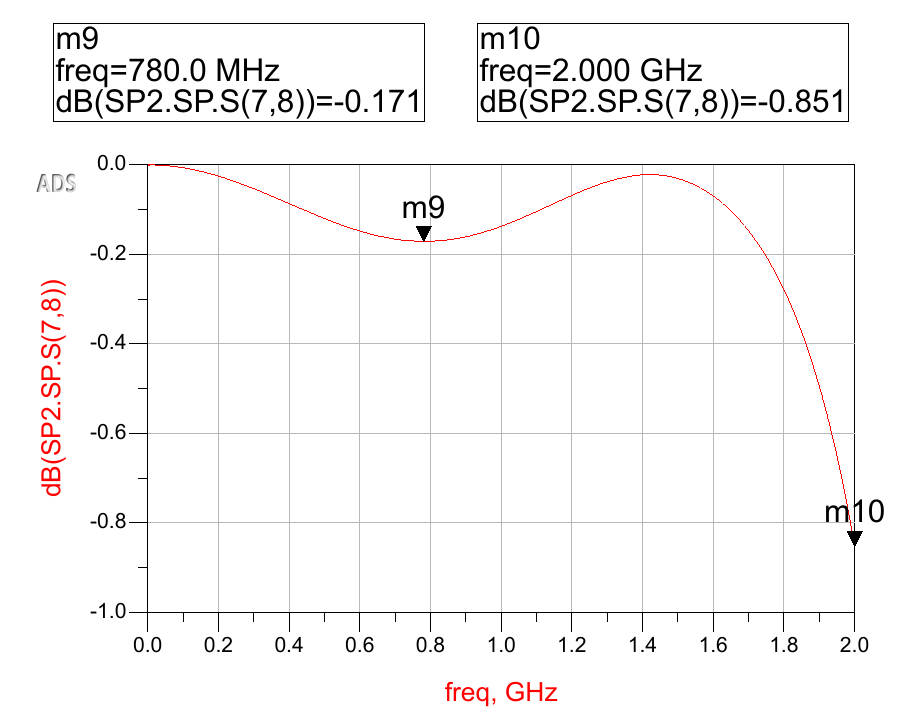
\includegraphics[width=\textwidth]{photo/passe_bas_vic/simu_zoom_passe_bas_distribue_ameliore.PNG}
		\caption{Avec zoom sur la bande passante}
		\label{fig:simu_zoom_passe_bas_distribue_ameliore}
	\end{subfigure}
	\caption{Simulation du module de S21 en dB du filtre de Tchebychev amélioré avec un stub}
	\label{fig:simu_passe_bas_distribue_ameliore}
\end{figure}


Comme prévu, on note la présence d'un 0 de transmission sur la fréquence 7 GHz. Le comportement en bande passante est similaire à celui du filtre sans le stub bien qu'il ne reste toujours pas conforme avec le gabarit. On remarque cependant que la bande atténuée du gabarit est respecté sur la bande $[3 GHz; 7,6 GHz]$ contre $[3GHz; 6,5 GHz]$ avec le filtre sans le stub. L'ajout d'un stub sur le filtre est donc une méthode viable pour augmenter la plage de fréquence de la bande atténuée qui respecte le gabarit du cahier des charges.



\subsection{Comparaison de différents substrats}

Dans cette partie on cherche à comparer la réponse d'un filtre de Tchebychev en technologie micro ruban sur un substrat epoxy et un substrat teflon. Le gabarit du filtre sera le même que pour les parties précédentes. Le schéma du filtre considéré est celui de la figure \ref{fig:schema_distribue_passe_bas_ads}. En effet, on décide de ne pas comparer les substrats avec un stub car les filtres réels mis à notre disposition n'en possèdent pas.\\

Pour le substrat en teflon, le filtre et les valeurs ses paramètres sont identiques à ceux de la figure \ref{fig:schema_distribue_passe_bas_ads}.\\

Pour le substrat en epoxy on se base sur la permittivité relative effective obtenue lors de la partie caractérisation sur l'epoxy large a savoir 4,574. Cette nouvelle valeur nous implique de recalculer les dimensions de nos lignes de transmission. Pour le détail complet, se référer à la partie sur la transformation des éléments localisés en éléments distribués. Pour le remplacement des bobines on prendra une largeur de cuivre $w$ de 0,5 mm tandis que pour les condensateurs on prendra une largeur de 10 mm. Dans les deux cas on prendra une hauteur de cuivre $h$ de 1,58 mm. Le tableau ci-dessous récapitule les longueurs des lignes $l$ obtenues à partir des paramètres précédemment explicités.

\begin{table}[H]
	\centering
	\begin{tabular}{|c|c|c|c|c|}
		\hline
		$L1$ & $C1$ & $L2$ & $C2$ & $L3$  \\
		\hline
		7,072 mm & 6,861 mm & 12,174 mm & 6,861 mm & 7,072 mm \\
		\hline
	\end{tabular}
	\caption{Longueurs des lignes de transmission qui remplacent les composants localisés pour le substrat en epoxy}
	\label{tab:longueur_ligne_passe_bas_tche_epoxy}
\end{table}

Ces valeurs de lignes et connaissant les paramètres du substrat nous avons simuler la réponse en fréquence de ce filtre. La figure \ref{fig:simu_comparaison_substrat} montre le résultat de cette simulation superposé à la précédente simulation sur un substrat en teflon.


\begin{figure}[H]
	\centering
	\begin{subfigure}[b]{0.49\textwidth}
		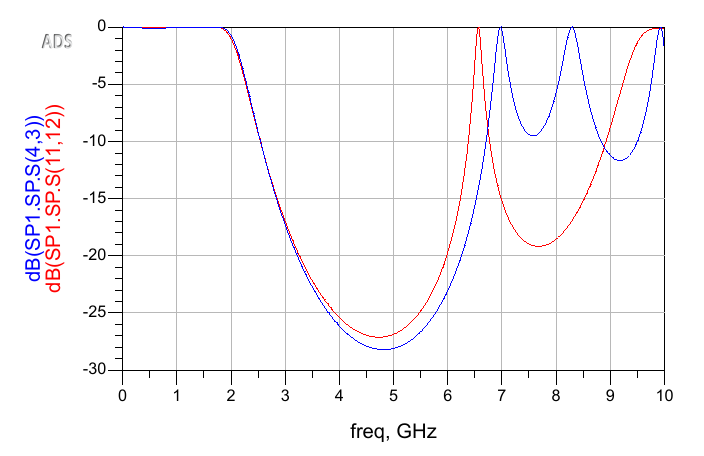
\includegraphics[width=\textwidth]{photo/passe_bas_vic/simu_comparaison_substrat.PNG}
		\caption{Sans zoom}
		\label{fig:simu_comparaison_substratG}
	\end{subfigure}
	\begin{subfigure}[b]{0.49\textwidth}
		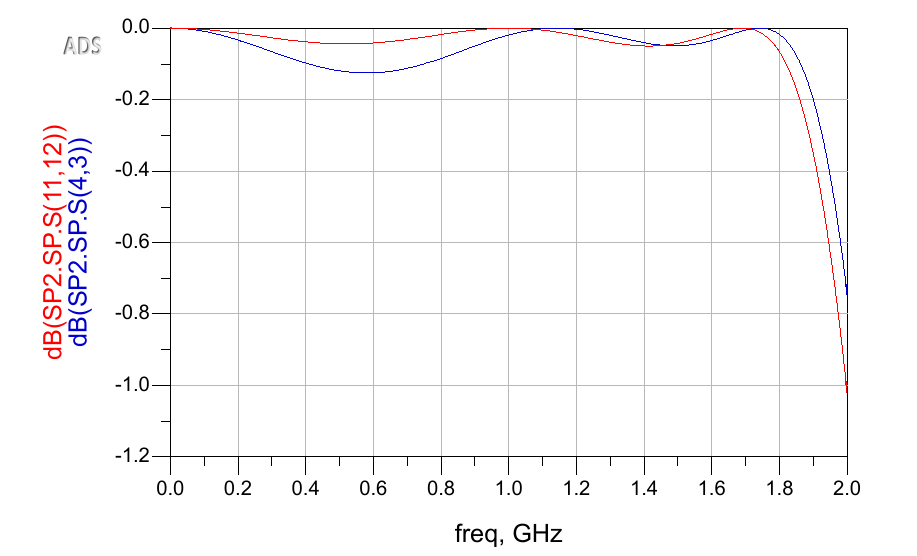
\includegraphics[width=\textwidth]{photo/passe_bas_vic/simu_zoom_comparaison_substrat.PNG}
		\caption{Avec zoom sur la bande passante}
		\label{fig:simu_zoom_comparaison_substrat}
	\end{subfigure}
	\caption{Simulation du module de S21 en dB pour des filtres de tchebychev en technologie micro ruban sur substrat epoxy en rouge et sur substrat teflon en bleu}
	\label{fig:simu_comparaison_substrat}
\end{figure}


On remarque que les différences entre le substrat en teflon et celui en epoxy ne sont presque pas visible dans la bande passante mais  qu'elles s'accentuent au fur et à mesure que les fréquences augmentent. Une chose très intéressante à noter et que nous avions déjà relevée lors de la partie sur la caractérisation du substrat : le teflon tient mieux les fréquences. Nous voulons entre par là que la fréquence de coupure du filtre sur epoxy se trouve légèrement inférieure à celle sur le substrat en teflon et il en va de même au niveau de la bande atténuée. En effet, la plage de fréquence où la bande atténuée du filtre respecte le gabarit est plus grande pour le substrat en teflon que celui en epoxy.


\subsection{Comparaison avec des filtres réels sur PCBs}

Pour finir cette partie sur le filtre passe-bas Tchebychev, nous souhaitons comparer nos résultats obtenus avec un filtre déjà réaliser sur PCB\footnote{PCB pour Printed Circuit Board en anglais ou circuit imprimé en français.}. Pour ce faire nous avons utilisé l'analyseur vectoriel mis à disposition pour relever les coefficients de transmission des filtres sur PCB. Le fichier en sortie de l'analyseur est avec une extension "s2p". Afin de les lire puis de les afficher sous ADS nous avons utilisé le schéma suivant.

\begin{figure}[H]
	\centering
	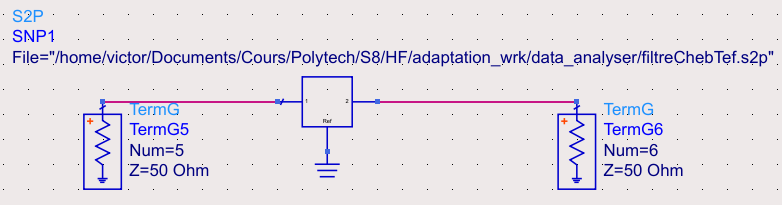
\includegraphics[width=10cm]{photo/passe_bas_vic/montage_filtre_reel_ADS.png}
	\caption{Schéma sous ADS pour lire les fichiers s2p.}
	\label{fig:montage_filtre_reel_ADS}
\end{figure}

Nous avons répliqué ce schéma une deuxième fois pour le substrat en epoxy puis nous avons lancé la simulation. La figure \ref{fig:simu_passe_bas_reel_tche} en est le résultat.

\begin{figure}[H]
	\centering
	\begin{subfigure}[b]{0.49\textwidth}
		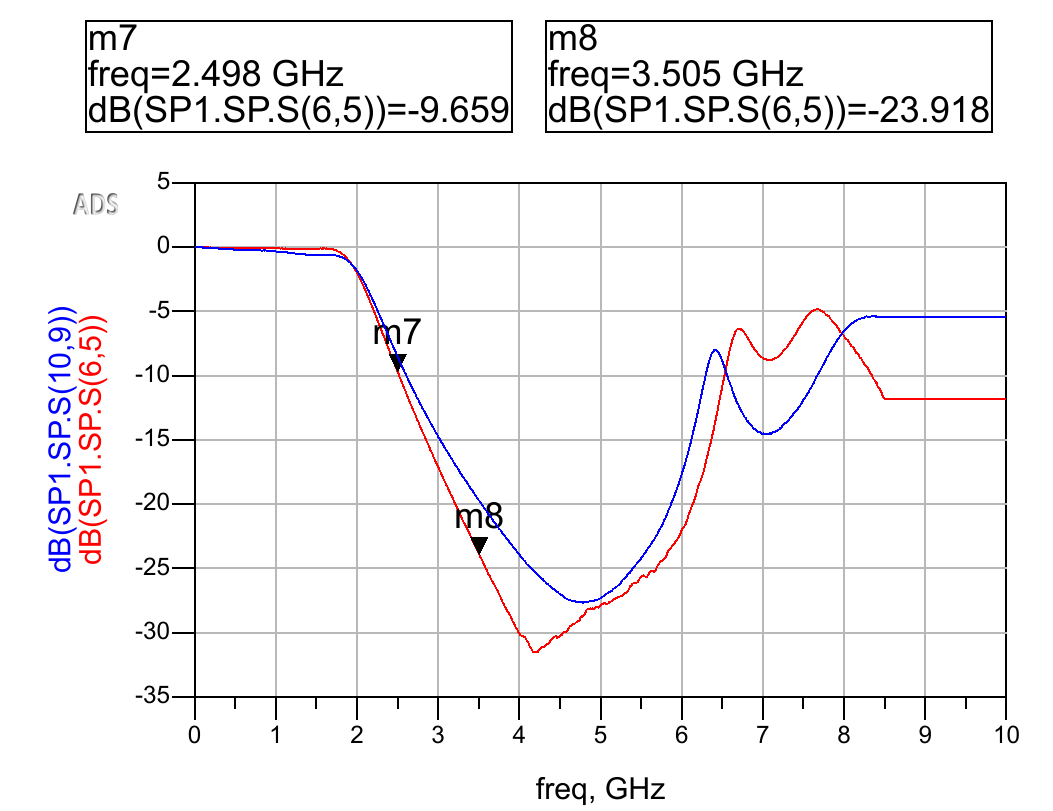
\includegraphics[width=\textwidth]{photo/passe_bas_vic/simu_passe_bas_reel_tche.PNG}
		\caption{Sans zoom}
		\label{fig:simu_passe_bas_reel_tcheG}
	\end{subfigure}
	\begin{subfigure}[b]{0.49\textwidth}
		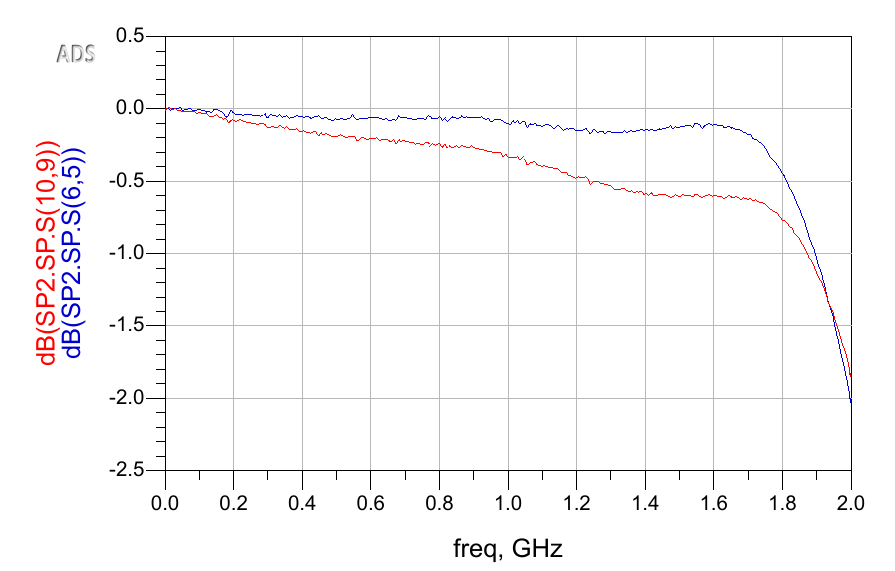
\includegraphics[width=\textwidth]{photo/passe_bas_vic/simu_zoom_passe_bas_reel_tche.PNG}
		\caption{Avec zoom sur la bande passante}
		\label{fig:simu_zoom_passe_bas_reel_tche}
	\end{subfigure}
	\caption{Module de S21 en dB pour un filtre de tchebychev en technologie micro ruban sur substrat epoxy en rouge et sur substrat teflon en bleu}
		\label{fig:simu_passe_bas_reel_tche}
\end{figure}


On observe un comportement similaire à la figure \ref{fig:simu_comparaison_substrat} avec l'ajout de perte liée au substrat lié au paramètre $tan(\delta)$. Comme lors de la partie précédente sur la comparaison des deux substrats on observe une fréquence de coupure pour l'epoxy légèrement inférieure à celle pour le teflon. On observe également une plage de fréquence plus faible pour l'epoxy que pour le teflon où la bande atténuée respecte le gabarit 



\newpage

\section{Synthèse d'un filtre passe-bas elliptique en technologie micro-ruban}

\subsection{Avant-propos : rappel du cahier des charges}

La partie qui suit consiste en la conception d'un second type de filtre passe-bande. Il s'agit d'un filtre passe-bas elliptique, également appelé filtre de Cauer selon la littérature. Un tel système possède diverses propriétés intéressantes. En effet, il s'agit d'un filtre avec une ondulation en bande passante mais également en bande atténuée. L'ondulation en bande atténuée présente à des fréquences particulières un gain en dB projeté vers $-\infty$. Il s'agit d'une propriété très intéressante car si le concepteur a la main sur ces fréquences particulières, celui-ci peut s'en servir pour grandement atténuer un quelconque signal nuisible. De plus, aucun autre filtre d'ordre égal peut avoir une raideur aussi importante que le filtre de Cauer. 
Le gabarit en atténuation fourni dans le cahier des charges est donné ci-dessous avec $f_c$ la fréquence de coupure du filtre à 2,5 GHz.

\begin{figure}[H]
	\centering
	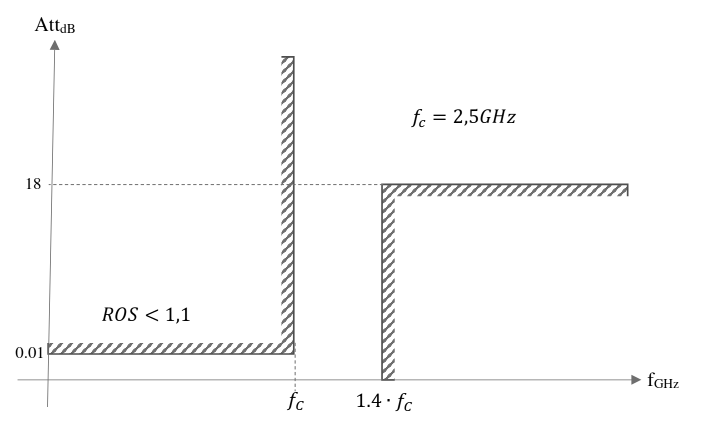
\includegraphics[width=10cm]{../3synthPBas/elliptique/gabarit_passe-bas_elliptique.png}
	\caption{Gabarit du filtre passe-bas elliptique imposé par le cahier des charges}
	\label{fig:gabarit_elliptique}
\end{figure}

Le cahier des charges contient également une table de valeurs pour la détermination du filtre passe-bas elliptique normalisé. Le choix de la ligne est effectuée en fonction des spécifications données sur le gabarit. Il est demandé par exemple une atténuation maximale $A_{max}$ en bande passante de 0,01 dB et un ROS (Rapport d'ondes stationnaires) n'excédant pas 1,1. La ligne choisie dans le nomogramme est donnée ci-dessous.

\begin{table}[H]
	\centering
	\begin{tabular}{|c|c|c|c|c|c|c|c|c|c|c|}
		\hline
		$A_{max}$(dB) & $VSWR$ & $\Omega$ & $A_s$(dB) & $g_1$ & $g_2$ & $g_3$ & $g_4$ & $g_5$ & $g_6$ & $g_7$\\
		\hline
		0.01 & 1.10 & 1.41 & 30.2 & 0.6265 & 0.1920 & 1.109 & 1.270 & 0.6535 & 0.7125 & 0.3441\\
		\hline
	\end{tabular}
	\caption{Nomogramme pour la détermination du filtre passe-bas elliptique normalisé}
	\label{tab:nomogramme_elliptique}
\end{table}

L'ensemble des $g_k$ formera un filtre respectant le gabarit imposé. Il s'agit des quatre premiers paramètres qui justifient le choix de ces valeurs. En effet l'atténuation maximale en bande passante est de 0,01 dB comme exigé sur le cahier des charges. Le VSWR (\textit{Voltage standing wave ratio}) est un paramètre inconnu mais simplement de nom. En réalité il s'agit du ROS, un critère à maîtriser afin d'éviter une importante réflexion qui mènerait à une perte de puissance. Le ROS est fixé à 1,10 c'est-à-dire que sur l'ensemble de la puissance transmise, 99,8\% est pour la charge et 0,2\% de la puissance est réfléchie. Ce paramètre semble peut-être anecdotique mais il peut s'avérer très important dans certaines applications. Par exemple, une puissance réfléchie trop élevée brûlerait le circuit et provoquerait la destruction du composant. Le paramètre $A_s$ donnera une atténuation minimale en bande atténuée de 30,2 dB, ce qui satisfait amplement le cahier des charges. Par ailleurs, la dernière variable $\Omega$ garantit qu'à la fréquence de 1,41$f_c$, la valeur $A_s$ sera atteinte.

\newpage

\subsection{Synthèse du filtre passe-bas elliptique en éléments localisés}

Dans cette section, il s'agit de synthétiser le filtre passe-bas elliptique en éléments localisés, c'est-à-dire avec des selfs et des capacités. Le cahier des charges offre le choix entre le filtre passe-bas en topologie impédance ou admittance. Le choix de l'un par rapport à l'autre n'apportera aucune différence sur le comportement fréquentiel. Afin de respecter le modèle d'équivalence tronçon de ligne - éléments localisés en technologie micro-ruban, la topologie impédance est choisie car le modèle suggère que les capacités doivent être tirées à la masse. Cependant, une publication IEEE (\textit{Institute electrical and electronics engineers}) propose la conception en micro-ruban de filtres elliptiques topologie admittance à l'aide d'une ligne symétrique à deux coudes et d'une capacité interdigitée.

\begin{figure}[H]
	\centering
	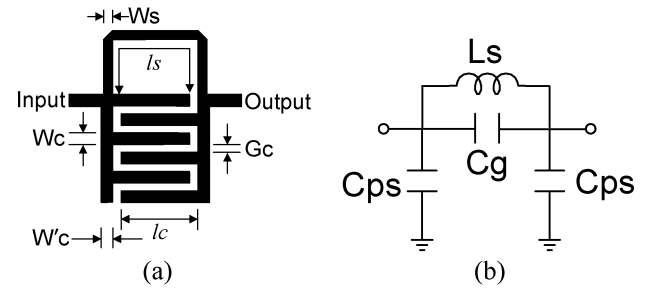
\includegraphics[width=9cm]{../3synthPBas/elliptique/solution_admittance.png}
	\caption{Topologie admittance du filtre elliptique en éléments localisés (b) et de son équivalent en technologie micro-ruban}
	\label{fig:elliptique_IEEE}
\end{figure}

\vspace{-1cm} %retrecissement pour que tout rentre sur une page

\begin{figure}[H]
	\centering
	\begin{circuitikz}
		\ctikzset{inductors/scale=0.9,inductor=american}
		\draw (0,2)
		to[L=$g_1$] (2,2)
		to[L=$g_2$] (2,0)
		to[C=$g_3$]	(2,-1) node[ground]{}
		(2,2)to[L=$g_4$] (4,2)
		to[L=$g_5$] (4,0)
		to[C=$g_6$]	(4,-1) node[ground]{}
		(4,2)to[L=$g_7$] (6,2);
	\end{circuitikz}
	\caption{Schéma prototype d'un filtre passe-bas de Cauer en topologie impédance}
\end{figure}

La structure a été décrite sous ADS, en passant des éléments $g_k$ normalisés aux valeurs de selfs et de capacités. Celle-ci est disponible dans la figure ci-dessous.

\begin{figure}[H]
	\centering
	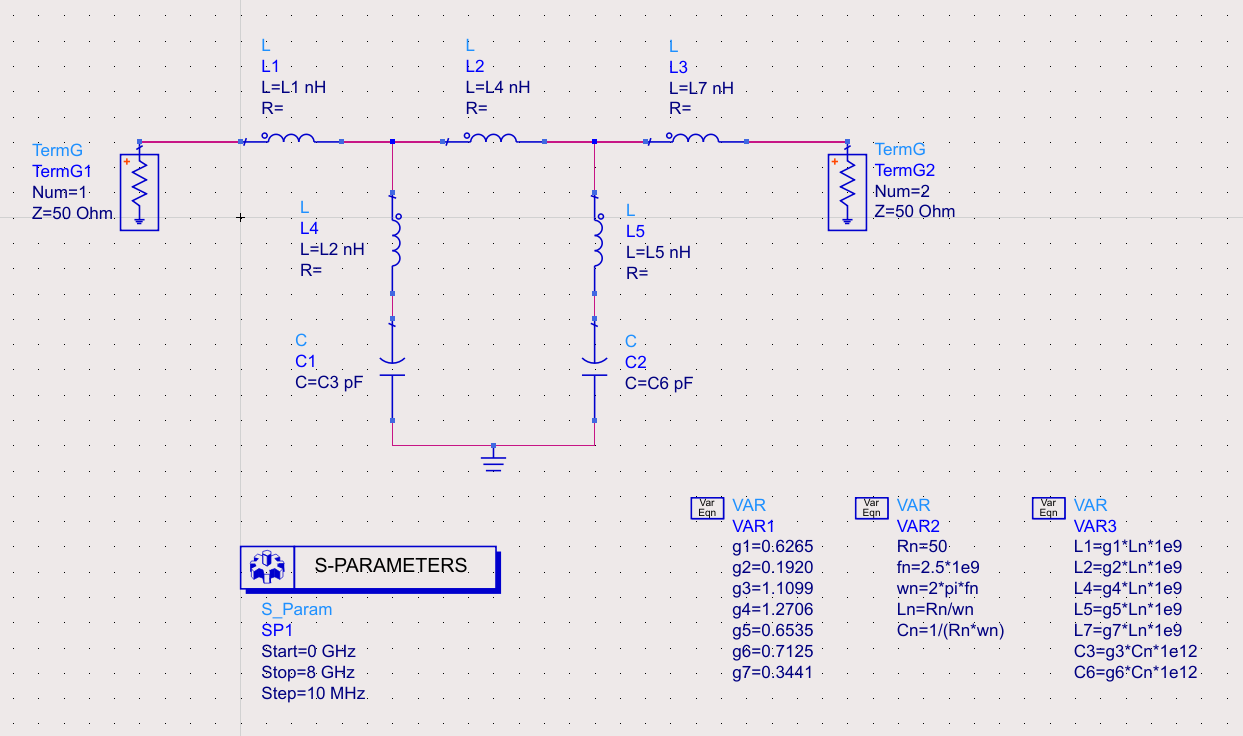
\includegraphics[width=12cm]{../3synthPBas/elliptique/modele_ADS_elliptique.png}
	\caption{Structure du filtre passe-bas elliptique en impédance sous ADS}
	\label{fig:montage_ADS_elliptique}
\end{figure}

\newpage

\subsection*{Validations}

La sous-section qui suit s'intéresse à valider la conception du filtre passe-bas elliptique en éléments localisés avant la transposer en lignes micro-rubans. La simulation sous ADS est effectuée entre 0 et 8 GHz. Le résultat de la simulation est donné dans la figure (\ref{fig:validation_elliptique_localise}) ci-dessous. Le graphique à gauche représente la réponse du filtre sur l'ensemble de la plage fréquentielle simulée. Celui de droite est compris entre 0 et 3 GHz, il s'agit d'un agrandissement effectué pour visualiser la réponse dans la bande passante.\\
En ce qui concerne la bande atténuée, l'atténuation minimale est de 30,133 dB bien supérieure au 18 dB exigé dans le cahier des charges, ce qui laisse une marge d'environ 12 dB. La bande passante n'offre pas le comportement désiré. En effet, l'atténuation maximale $A_{max}$ dépasse à quelque $10^{-3}$ près des 0,01 dB souhaité. Également à la fréquence de coupure $f_c$, le gain est de -0,012 dB et non de -0,01 dB.\\
Il pourrait être intéressant de réaliser une simulation en mode tuning et régler les $g_k$ pour obtenir le comportement en bande passante désiré.

\begin{figure}[H]
	\centering
	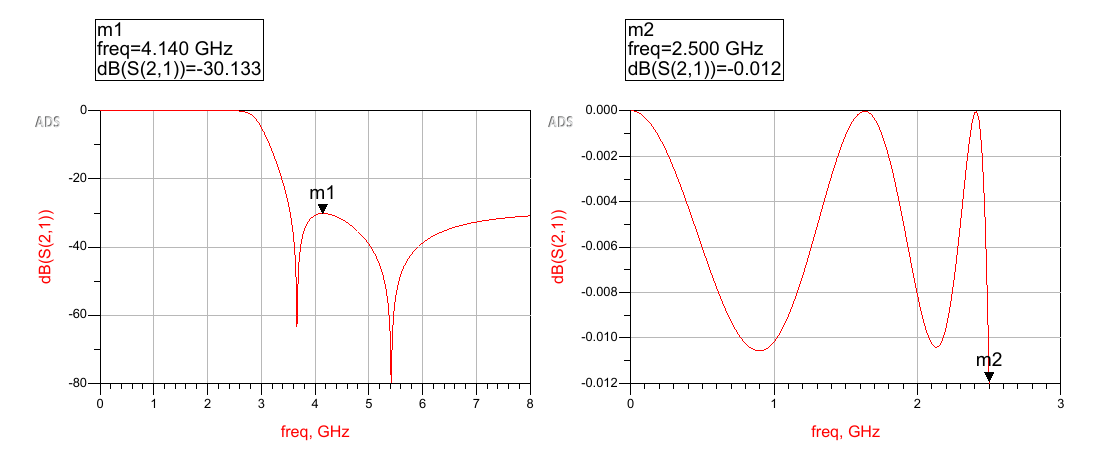
\includegraphics[width=16cm]{../3synthPBas/elliptique/filtre_elliptique_localise.png}
	\caption{Graphique représentant l'évolution du gain en dB du filtre passe-bas elliptique en éléments localisés en fonction de la fréquence}
	\label{fig:validation_elliptique_localise}
\end{figure}

\subsection{Transposition du filtre passe-bas elliptique en technologie micro-ruban}

Il s'agit dans cette section de transposer le filtre conçu précédemment en technologie micro-ruban. En respectant le modèle d'équivalence tronçon de ligne -  éléments localisés et ses hypothèses (il faut que $l \ll \lambda_g$,$Z_C \gg Z_0$ pour les inductances et $Z_C \ll Z_0$ pour les capacités), les selfs seront réalisées avec des petites largeurs et les capacités avec des largeurs $W$ plus élevées. La figure ci-dessous est un exemple de structure de ce filtre en micro-ruban présenté dans divers ouvrages. 

\begin{figure}[H]
	\centering
	\begin{circuitikz}[scale=0.8]
		\draw (-5,0) to (-4,0)
		to(-4,0.25) to (-1.75,0.25)
		to(-1.75,-1) to(-2.25,-1)
		to(-2.25,-2) to(-1,-2)
		to(-1,-1) to(-1.5,-1)
		to(-1.5,0.25) to(-0.25,0.25)
		to(-0.25,0) to (0.75,0);
		\draw (-5,0.75) to (-4,0.75)
		to(-4,0.5) to (-3,0.5)
		to(-3,2) to (-3.5,2)
		to(-3.5,3) to (-2.25,3)
		to(-2.25,2) to (-2.75,2)
		to (-2.75,0.5) to (-0.25,0.5)
		to(-0.25,0.75) to (0.75,0.75);
		\node at (-3.5,-0.1) {$L_1$};
		\node at (-2.4,1.2) {$L_2$};
		\node at (-1.9,2.4) {$C_3$};
		\node at (-2.2,-0.1) {$L_4$};
		\node at (-1.1,-0.4) {$L_5$};
		\node at (-0.6,-1.5) {$C_6$};
		\node at (-0.8,0.75) {$L_7$};
	\end{circuitikz}
	\caption{Schéma représentatif de la structure du filtre passe-bas elliptique en ligne micro-ruban}
	\label{fig:modele_elliptique_microstrip}
\end{figure}

\newpage

La conception du filtre passe-bas Tchebychev a respecté à la lettre l'ensemble de ce modèle d'équivalence y compris la relation d'ordre $l \ll \lambda_g$, hypothèse qui justifie la linéarisation du terme $\mbox{tan}(\beta l)$ dans la formule de l'impédance vue $Z_{vue}$. Cependant comme le montre la figure (\ref{fig:simu_passe_bas_distribue}), à partir d'une certaine fréquence la longueur d'onde guidée $\lambda_g$ est de l'ordre de la longueur $l$ de la ligne. La linéarisation de la tangente n'a plus de sens à partir de cette fréquence. Ainsi pour la suite du rapport et dans l'objectif d'obtenir un meilleur résultat, la linéarisation $\mbox{tan}(\beta l) \approx \beta l$ ne sera pas effectuée.\\

Il s'agit désormais de fixer les limites géométriques qui seront utilisées pour obtenir des lignes d'impédance caractéristique $Z_C$ faible ou élevée. Dans le cas d'impédance élevée ($Z_C \gg Z_0$ pour les inductances), la largeur de ligne $W$ sera fixée selon la technologie de gravure et sa précision. Les procédés de photolithographie choisis pour les plaques de test en laboratoire possèdent une limite de gravure de 0,50 mm. La largeur de ligne pour les inductances, notée $W_L$, sera donc de 0,50 mm.\\
En ce qui concerne les impédances faibles ($Z_C \ll Z_0$ pour les capacités), la largeur de ligne $W_C$ est définie par la relation $W_C = 0.1\lambda_g$ avec $\lambda_g$ la longueur d'onde guidée à la fréquence d'intérêt de 2,5 GHz. Une telle dimension géométrique pour la largeur évite l'excitation des modes supérieurs à des fréquences proches de $f_c$. Ces modes sont alors projetés plus dans le plan spectral et cela garantie l'utilisation d'un seul mode qui est le mode dominant. Il est possible de trouver un bon compromis entre ce critère et les limites de gravure. Pour la suite la largeur $W_C$ sera définie à 10 mm.\\

Les valeurs $W_L$ et $W_C$ étant déterminées, il s'agit à l'aide de la hauteur du substrat $h$ et de ses autres paramètres de déterminer les deux impédances $Z_{C_C}$ et $Z_{C_L}$ et constantes diélectriques relatives effectives $\varepsilon_{reffC}$ et $\varepsilon_{reffL}$. Le substrat considéré par la suite sera le verre téflon large. Ces calculs sont réalisés à partir de l'outil LineCalc intégré à ADS. La figure ci-dessous présente son interface. Celle-ci représente la détermination des paramètres $Z_{C_C}$ et $\varepsilon_{reffC}$ à l'aide des données du substrat et de $W_C$ à la fréquence $f_c$ de 2,5 GHz. Le paramètre \texttt{L} d'une valeur de 100 mm ici n'a aucune incidence sur la détermination de ces paramètres. En effet, $\varepsilon_{reffC}$ dépend de $\varepsilon_{r}$ et du rapport $h/W_C$. De même $Z_{C_C}$ ne dépend que de $\varepsilon_{r}$, $h$ et de $W_C$. Le bouton \texttt{Analyze} donne le résultat de \texttt{Z0} ($Z_{C_C}$) et de \texttt{K\_Eff} ($\varepsilon_{reffC}$) à partir des données déjà possédées. Ces deux valeurs sont retenues, puis l'opération est réitérée afin d'obtenir $Z_{C_L}$ et $\varepsilon_{reffL}$.

\begin{figure}[H]
	\centering
	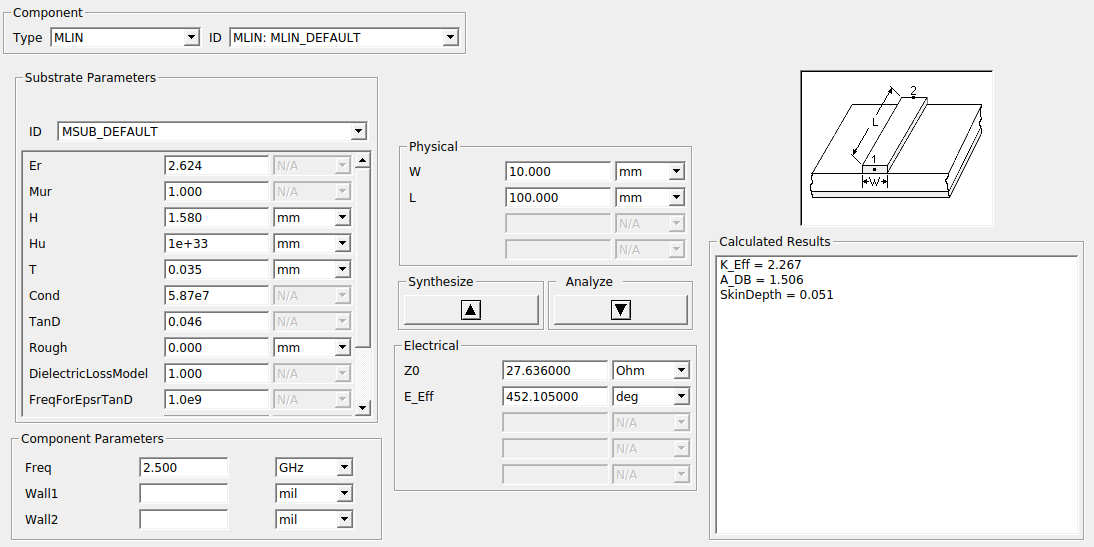
\includegraphics[width=16cm]{../3synthPBas/elliptique/exemple_linecalc.png}
	\caption{Présentation de l'interface LineCalc (exemple avec la détermination de $\varepsilon_{reffC}$ et $Z_{C_C}$)}
	\label{fig:interface_linecalc}
\end{figure}

\newpage

Pour la suite, l'ensemble des équations suivantes peuvent être calculées avec les grandeurs données par LineCalc. Ces diverses relations sont inscrites dans ADS. La valeur $c$ correspond ici à la célérité de la lumière.

\begin{equation}
	\lambda_{g_C}=\frac{c}{f_c \sqrt{\varepsilon_{reffC}}} \mbox{ et } \lambda_{g_L}=\frac{c}{f_c \sqrt{\varepsilon_{reffL}}}
\end{equation}

\begin{equation}
	\beta_C = \frac{2 \pi}{\lambda_{g_C}} \mbox{ et } \beta_L = \frac{2 \pi}{\lambda_{g_L}}
\end{equation}

Et les longueurs $l_C$ et $l_L$ définies comme :

\begin{equation}
	l_C= \frac{1}{\beta_C} \mbox{arctan}\big(2 \pi f_c Z_{C_C} C\big) \mbox{ et } l_L= \frac{1}{\beta_L} \mbox{arctan}\big(\frac{2 \pi f_c L}{Z_{C_L}}\big)
\end{equation}

\vspace{2cm}

La figure (\ref{fig:structure_elliptique_microstrip}) représente la structure utilisée sur ADS pour l'implémentation du filtre elliptique en technologie micro-ruban. L'ensemble des équations ci-dessus ont été écrites à l'aide de la directive \texttt{VAR}. Les composants \texttt{MLIN} représentent les lignes dont les longueurs et largeurs ont été déterminées précédemment. Les composants \texttt{MTEE} (\textit{T-junction}) et \texttt{MSTEP} (\textit{Step in width}) affinent la structure en prenant en compte les discontinuités. En effet, le \texttt{MSTEP} prends en compte la transformation d'impédance provoquée par le changement brusque de largeur de ligne. En ce qui concerne le composant \texttt{MTEE}, celui-ci prends en compte une discontinuité de la distribution du champ $\overrightarrow{E}$, provoquée par la forme coudée de la ligne.

\begin{figure}[H]
	\centering
	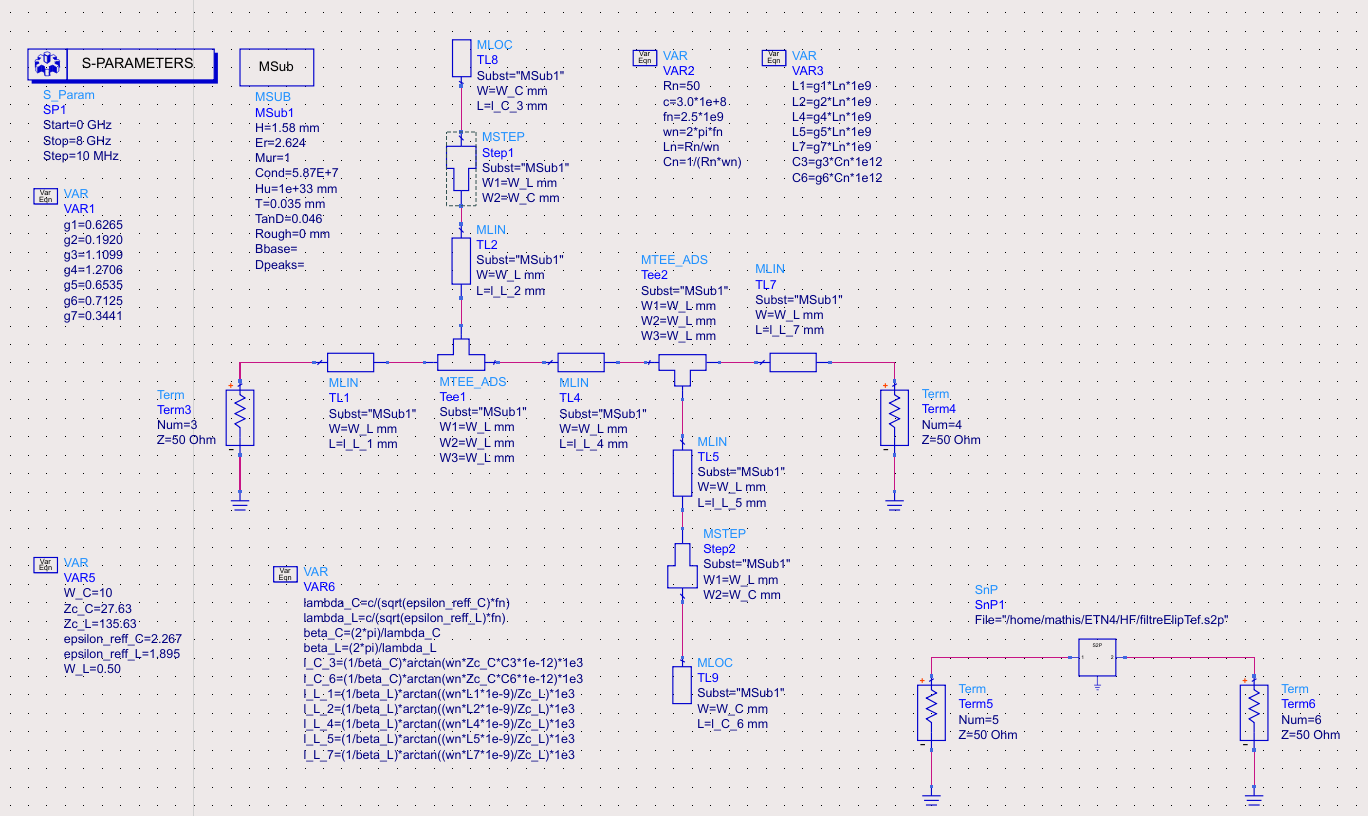
\includegraphics[width=14cm]{../3synthPBas/elliptique/modele_microstrip_ADS.png}
	\caption{Montage du filtre elliptique en ligne micro-ruban sur ADS}
	\label{fig:structure_elliptique_microstrip}
\end{figure}

\newpage

\subsection*{Validations}

Il s'agit dans cette sous-section de simuler le comportement du filtre elliptique en technologie micro-ruban. La simulation est réalisée dans un intervalle de fréquence de 0 à 8 GHz. La figure (\ref{fig:resultat_elliptique_microstrip}) précise le résultat de la simulation. La courbe rouge représente les mesures réalisées en laboratoire à l'aide du VNA sur verre téflon. La courbe bleue correspond au résultat du filtre structuré sur ADS. Le graphique de gauche est l'ensemble de la réponse sur la gamme de fréquence de simulation. Le graphique de droite est un agrandissement sur la bande passante.


\begin{figure}[H]
	\centering
	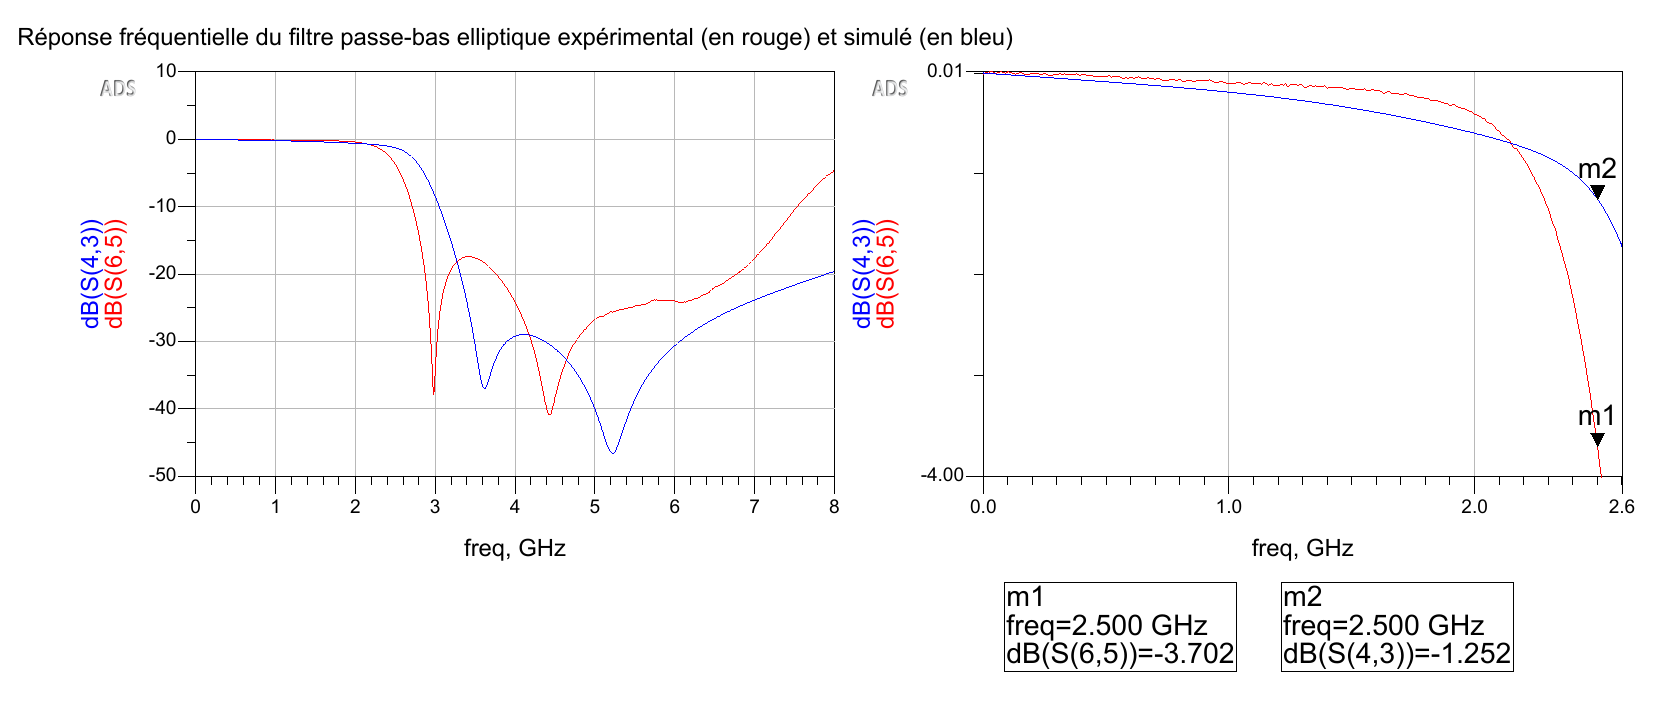
\includegraphics[width=16cm]{../3synthPBas/elliptique/resultat_simu_microstrip.png}
	\caption{Graphique de la réponse fréquentielle du filtre simulé et des mesures expérimentales du filtre elliptique fourni au laboratoire}
	\label{fig:resultat_elliptique_microstrip}
\end{figure}

Il est possible de remarquer la présence d'une ondulation en bande atténuée, élément caractéristique d'un filtre de Cauer. La bande atténuée commence à la fréquence de 3,5 GHz, à cette fréquence le gain est de -30 dB ce qui valide le cahier des charges avec une marge de 12 dB d'atténuation. Une remontée en gain s'effectue ensuite mais reste en dessous des 18 dB d'atténuation minimale exigé. Une telle remontée est provoquée par le changement de comportement des inductances et des capacités à des fréquences particulières. Néanmoins, cette remontée est rendue bien moins abrupte grâce à la non-linéarisation de la tangente (non respect de l'hypothèse $l \ll \lambda_g$ car n'est plus valable à partir d'une certaine fréquence).\\
À comparer avec le résultat expérimental, la courbe de la simulation est en dessous de la rouge en bande atténuée. Le comportement en bande atténuée respecte davantage le cahier des charges que le filtre réalisé sur plaque en laboratoire. Cela pourrait s'expliquer par un angle de perte utilisé en simulation de 0,046 c'est-à-dire le double d'un angle de perte classique d'un diélectrique verre téflon. Il s'agirait également de cette mauvaise estimation de la tangente de perte $\mbox{tan}(\delta)$ qui provoquerait une descente brutale du gain en bande passante. Le cahier des charges n'est pas valide en ce qui concerne la bande passante.\\


\newpage

\section{Synthèse d'un filtre passe-bande}

La synthèse d'un filtre en hautes-fréquences à partir d'un gabarit se rapporte à la méthode étudiée en moyenne fréquence. Une étape finale est ajoutée permettant la transformation des éléments localisés en éléments distribués.
Le cahier des charges est le suivant, concevoir un filtre passe bande basé sur une fonction d'approximation de type Tchebychev et respectant le gabarit figure \ref{fig:gab}. L'implémentation réelle doit se en utilisant exclusivement des lignes micro-ruban de longueur $\lambda_g/2$ ou $\lambda_g/4$ et des stubs.

\begin{figure}[H]
	\centering
	\includegraphics[width=0.5\linewidth]{ressources/gabarit_passe_bande}
	\caption{Gabarit du filtre passe-bas souhaité}
	\label{fig:gab}
\end{figure}
Les valeurs numériques associées au gabarit sont les suivantes. Les fréquences sont en GHz et l'atténuation en dB. 
	\begin{table}[H]
		\centering
\begin{tabular}{|c|c|c|c|c|c|}
		\hline
	$A_{max}$& $A_{min}$ & $f_c^-$ & $f_s^-$ & $f_s^+$ &$f_c^+$ \\ \hline
	0,1000	 & 15,00 		& 1,500	   & 1,750 & 2,250& 3,000 \\ \hline
	\end{tabular}
\caption{Valeur numérique gabarit souhaité}
	\end{table}
\subsection{Symétrie du gabarit}
Avant de commencer la synthèse du filtre il est nécessaire de valider une condition sur la symétrie. Si elle n'est pas respectée il faudra modifier le gabarit du cahier des charges. La condition s'opère sur la moyenne géométrique de la bande passante et de la bande coupée notées :
\begin{equation}
	 f_{co} = \sqrt{f_c^-.f_c^+}, \quad f_{so} = \sqrt{f_s^- f_s^+}
\end{equation}
Ainsi, si $f_{so} = f_{co}$, le gabarit est centré il n'est pas nécessaire de réaliser d'opération particulaire. On obtient a alors  $f_{so} = f_{co} = f_0$ avec $f_0$ la fréquence centrale du gabarit. Si $f_{so} \neq f_{co}$, le gabarit n'est pas centré il faut passer par une étape de centrage du gabarit avant de réaliser la synthèse du filtre.\\
Application numérique :\\
\begin{equation}
f_{co} = \sqrt{f_c^-.f_c^+} = \sqrt{1,500*3,000} = 2,121 GHz
\end{equation}
\begin{equation}
	f_{so} = \sqrt{f_s^- f_s^+} = \sqrt{1,750*2,250} = 1,984 GHz
\end{equation}
\begin{equation}
f_{so} <	f_{co}
\end{equation}
Le filtre est asymétrique il faut réaliser l'opération de centrage. Dans notre cas elle vise à diminuer $f_{co}$. Il est possible de faire varier la borne positive $f_c^+$. Cela a pour effet de sur-contraindre le cahier des charges. Pour répondre aux exigences il est interdit d'élargir la bande atténué ou de diminuer la bande passante. Ainsi on fixe la fréquence centrale $f_0 = f_{so} = \sqrt{f_s^- f_s^+}$.  
Il vient donc :
\begin{equation}
f_c^+=\frac{f_{so}^2}{f_c^-}=\frac{1,984^2}{1,500}=2,614GHz
\end{equation}
Les nouvelles valeurs numériques pour le gabarit du filtre sont les suivantes. Elle font référence à la figure \ref{fig:gab}.
	\begin{table}[H]
	\centering
	\begin{tabular}{|c|c|c|c|c|c|c|}
		\hline
		$A_{max}$& $A_{min}$ & $f_c^-$ & $f_s^-$ & $f_0$ & $f_s^+$ &$f_c^+$ \\ \hline
		0,1000		 & 15,00 		& 1,500	   & 1,750 & 1,984 & 2,250& 2,614 \\ \hline
	\end{tabular}
	\caption{Valeur numérique gabarit centré}
\end{table}
\subsection{Gabarit passe-bas}
L'étape suivante dans la conception d'un filtre passe-bande symétrique vise à simplifier la synthèse en passant par un gabarit passe-bas. Cela permet de calculer son ordre puis sa structure en éléments localisés.
\begin{figure}[H]
	\centering
	\includegraphics[width=0.5\linewidth]{ressources/gabarit_passe_bas}
	\caption{Gabarit filtre passe-bas équivalent}
	\label{fig:gabaritpassepas}
\end{figure}
L'évaluation du coefficient de sélectivité permet d'établir le gabarit normalisée. Cette grandeur se note $k$ est sans unité et strictement inférieure à 1. Son expression est la suivante :
\begin{equation}
	k=\frac{\Delta.f_s}{\Delta.f_c}=\frac{f_s^+-f_s^-}{f_c^+-f_c^-}=\frac{2,250-1,75}{2,614-1,500}=0,4488
\end{equation}
L'ordre du filtre $\delta \in N$ est donné pour une fonction d'approximation de Tchebychev avec l'expression suivante. Les atténuations $A_{min}$ et $A_{max}$ en dB correspondent respectivement aux fréquences $f_s$ et $f_c$.
\begin{equation}
\delta \geq \frac{argch
	\Big( \sqrt{\cfrac{10^{A_{min}/10}-1}{10^{A_{max}/10}-1}}
	\Big)
}{argch(1/k)}
\end{equation}
On rappelle pour la calculatrice :
\begin{equation}
argch(x)=ln(x+\sqrt{x^2-1})
\end{equation}
On calcule avec $A_{min} = 15dB$ et $A_{max} = 0,1dB$. L'ordre $\delta$ est arrondi à l'entier supérieur.
\begin{equation}
\frac{argch
	\Big( \sqrt{\cfrac{10^{15/10}-1}{10^{0,1/10}-1}}
	\Big)
}{argch(1/0,4488)} = 2,975, \quad \delta = 3
\end{equation}
Le gabarit impose un ordre minimum de 3, c'est la valeur que nous retiendront. On note tout de même que l'arrondi au supérieur présente un faible écart avec l'ordre choisi. Notre filtre devrait respecter les spécifications mais des approximations pourraient entraîner des débordements notamment aux fréquences particulières $f_c$ et $f_s$.
\subsection{Prototype passe-bas normalisé vers passe-bande dénormalisé}
Cette étape vise à transformer le schéma passe-bas en son équivalent passe bande. Il existe deux schémas possibles dit de type impédance et de type admittance où, respectivement, le premier élément est une inductance ou un condensateur. Le cahier des charges ne donne pas d'indications sur ce point. Nous choisirons le schéma qui a l'avantage de simplifier la transposition micro-ruban.
\begin{figure}[H]
	\centering
	\begin{circuitikz}[scale=0.8]
		\draw 
		(0,0) to[esource] (0,2) % The voltage source
		to [R=$1$] (3,2) 
		to[L=$l'_1$] (5,2)
		to[L=$l'_3$] (8,2)
		to [R=$r$] (8,0) 
		to[short] (0,0)
		(5.3,2)to[C=$c'_2$] (5.3,0);
	\end{circuitikz}
	\caption{Schéma prototype filtre passe-bas ordre 3 en impédance}
	\label{fig:ordre3_LP_adm}
\end{figure}
La figure \ref{fig:ordre3_LP_adm} représente le prototype du filtre passe-bas. Il est composé de trois composants réactifs et le premier est une self, nous sommes bien en présence d'un filtre d'ordre trois de type impédance. Les valeurs normalisées de ces composants s'expriment à partir de l'atténuation maximum $A_{max}$, de l'ordre du filtre et de la charge. Dans le cas des ordres pairs les deux résistances n'ont pas la même valeur, il est donc préférable de choisir un ordre impair sans quoi une problématique d'adaptation se posera. Les calculs pour obtenir les valeurs des composants sont détaillés dans \cite{cours_MF} à la page 93. Ils font intervenir des fonctions trigonométriques relativement complexes. La figure \ref{fig:coefnormaliseondulation01db} ci-dessous rassemble ces grandeurs et nous évitent les calculs. Elle correspond à une ondulation inférieure à 0,1dB en bande passante et un ordre compris entre 1 et 10. 
\begin{figure}[H]
	\centering
	\includegraphics[width=0.8\linewidth]{ressources/coef_normalise_ondulation01dB}
	\caption{Coefficients normalisés fonction de Tchebychev 0,1dB ondulation}
	\label{fig:coefnormaliseondulation01db}
\end{figure}
La première colonne de ce tableau correspond à l'ordre du filtre. Les valeurs suivantes correspondent aux composants de gauche à droite sur le schéma. La dernière valeur concerne la résistance de charge. On remarque bien que pour les ordres impairs cette dernière vaut l'unité contrairement aux ordres impairs. Dans notre cas $l'_1=1,0315$, $c'_2=1,1474$ et $l'_3=1,0315$. Les informations nécessaires à la transformation du schéma équivalent passe-bas au schéma équivalent passe-bande ont été rassemblés. Nous pouvons opérer cette opération. Les éléments inductifs doivent être remplacés par une self et un condensateur en série. Les éléments capacitifs doivent être remplacés par une self et un condensateur en parallèle. Les valeurs normalisées des nouveaux composants sont données par les expressions suivantes:\\
Cas de l'inductance :
\begin{equation}
c_k=\frac{B}{l'_k}, \quad l_k=\frac{l'_k}{B}, \quad k = \{1,3\}
\end{equation}
Cas du condensateur :
\begin{equation}
c_k=\frac{c'_k}{B}, \quad  l_k=\frac{B}{c'_k}, \quad k = \{2\}
\end{equation}
Où B désigne la bande passante
\begin{equation}
	B=\frac{\Delta f_s}{f_0}=\frac{f_s^+-f_s^-}{f_0}=\frac{2,250-1,75}{1,984}=0,2520
\end{equation}
Le schéma du filtre passe-bande en éléments localisés après transformation est illustré par la figure \ref{fig:ordre3_BP_imp}.

\begin{figure}[H]
	\centering
	 \ctikzset{bipoles/length=1.1cm}
	\begin{circuitikz}[scale=0.85]
		\draw 
		(0,0) to[esource] (0,3) % The voltage source
		to [R=$1$] (2,3) 
		to[L=$l_1$] (4,3)
		to[C=$c_1$] (6,3)
		to[L=$l_3$] (8,3)
		to[C=$c_3$] (10,3)
		to [R=$r$] (10,0) 
		to[short] (0,0)
		(6,3) to[short] (6,2.5)
		(5.5,2.5) to[short] (6.5,2.5)
		(5.5,2.5) to[L=$l_2$] (5.5,0.5)
		(6.5,2.5) to[C=$c_2$] (6.5,0.5)
		(5.5,0.5) -- (6.5,0.5)
		(6,0.5) -- (6,0);
	\end{circuitikz}
	\caption{Schéma filtre passe-bande ordre 3 type impédance en éléments localisés}
	\label{fig:ordre3_BP_imp}
\end{figure}
À partir des expressions précédentes il est possible de calculer les valeurs normalisées de ces nouveaux composants. Nous pouvons par la même occasion opérer la dénormalisation. Les grandeurs dénormalisées seront notées en majuscule. De nouveau on s'appuis sur le cours d'électrique moyennes fréquences \cite{cours_MF}. On y extrait les égalités suivantes :
\begin{equation}
C_k = \frac{c_k}{2\pi f_0.R}
\quad
L_k = \frac{l_k.R}{2\pi .f_0}
\quad
k=\{1,2,3\}
\end{equation}
On prendra la résistance de charge valant $50\Omega$ et la fréquence centrale $f_0$ 1,984GHz. Un petit programme Octave nous permet d'automatiser ce calcul. Les résultats de l'étape de transformation et de dénormalisation sont rassemblés dans le tableau \ref{tab:denorm_BP}. On rappelle que la notation utilisée représente les grandeurs normalisées en minuscule et les grandeurs dénormalisées en majuscule.

\begin{table}[H]
	\centering
	\begin{tabular}{|c|c|c|c|}
		\hline
		k & 1 & 2 & 3 \\
		\hline
		$c_k$ & 0,2443 & 4,553 & 0,2443 \\ \hline
		$l_k$ &	4,093	&	0,2196	&	4,093	\\ \hline
		$C_k$ &	0,3917pF&	7,307pF	&	0,3917pF\\ \hline
		$L_k$ &	16,42nH	&	0,8804nH& 16,42nH	\\ \hline
	\end{tabular}
	\caption{Valeurs passe-bande avant et après dénormalisation}
	\label{tab:denorm_BP}
\end{table}
%\begin{table}[H]
%	\centering
%	\begin{tabular}{|c|c|c|c|}
%		\hline
%		k & 1 & 2 & 3 \\
%		\hline
%		$c_k$ & 0,2443 & 4,553 & 0,2443 \\ \hline
%		$l_k$ &	4,093	&	0,2196	&	4,093	\\ \hline
%		$C_k$ &	0,3919pF&	7,303pF	&	0,3919pF\\ \hline
%		$L_k$ &	16,41nH	&	0,8808nH& 16,41nH	\\ \hline
%	\end{tabular}
%	\caption{Valeurs passe bande avant et après dénormalisation}
%	\label{tab:denorm_BP}
%\end{table}
Afin de valider les valeurs obtenues nous pouvons recourir à une simulation sur ADS. Le schéma tracé est illustré par la figure \ref{fig:ads_sch_BP_localise}.
\begin{figure}[H]
	\centering
	\includegraphics[width=0.8\linewidth]{../4synthPBande/impedance/schema_passe_bande_localise}
	\caption{Schéma filtre passe-bande ordre 3 type impédance en éléments localisés sous ADS}
	\label{fig:ads_sch_BP_localise}
\end{figure}
Il fait intervenir des composants de la bibliothèque "lumbed component". La simulation porte sur l'observation des paramètres S et plus particulièrement du coefficient de transition $S_{21}$. Le résultat obtenu est donné par la figure \ref{fig:ads_S21_BP_localise1}. Elles permettent respectivement de vérifier la coupure et l'ondulation en bande passante.
\begin{figure}[H]
	\centering
	\includegraphics[width=0.49\linewidth]{../4synthPBande/impedance/S21__passe_bande_localise}
	\includegraphics[width=0.49\linewidth]{../4synthPBande/impedance/S21__bande_passante_passe_bande_localise}
	\caption{Simulation du module de S21 pour passe bande localisé en dB}
	\label{fig:ads_S21_BP_localise1}
\end{figure}
La figure de gauche représente le paramètre S21 en db sur la bande spécifiée par le gabarit. On relève une atténuation de 15,58dB et 14,97dB aux points m1 et m4. Seul le premier respecte strictement le cahier des charges. La figure de gauche représente elle aussi le coefficient de transition mais sur une bande plus étroite correspondant à la bande passante. La condition du gabarit spécifie une ondulation inférieure à 0,1dB. Elle est respectée partout sauf aux points m5 où on relève 0,101dB. Les résultats de cette simulation présentent deux débordements aux fréquences particulières $f_c^-$ et $f_s^-$. Cela s'explique par une approximation réalisée lors du centrage du gabarit. En effet, seule la borne $f_c^+$ a été déplacée ce qui entraîne une légère dissymétrie entre le gabarit initial et celui recentré. Aussi, nous avons pu remarquer que l'ordre du filtre décimal est très proche de la valeur entière retenue. Cela a pour effet de laisser peu de marge aux fréquences particulières. Ces deux éléments cumulés ont joué en notre défaveur et aboutie à une synthèse en limite de spécification. 
Il existe une méthode détaillée dans le \textit{cours de filtrage actif} de Vincent Gouret faisant varier à la fois $f_c^+$ et $f_c^-$ lors du recentrage. Cette méthode est plus complexe mais aurait probablement permise de réaliser une synthèse répondant parfaitement au gabarit.Les résultats de simulation restent malgré tout concluant car ils présentent une erreur très faible. Nous conserverons donc les valeurs des composants pour la suite des calculs.\\

Les valeurs dénormalisées obtenues devraient permettre en théorie de constituer un filtre passe-bande en éléments localisés. Cependant en pratique l'ordre de grandeur (0,1pF pour les condensateurs et 1nH pour les inductances) pose un problème de provisionnement. En effet, elles sont peu réalistes puisque comparables aux phénomènes parasites des boîtiers et conducteurs. Il est possible de résoudre ce problème en transformant cette synthèse localisé en synthèse distribuée.

\subsection{Transposition vers la technologie micro-ruban}
Il existe plusieurs circuits s'appuyant sur les propriété des lignes pour réaliser un filtre passe-bande. Nous en détaillerons deux basées uniquement sur des lignes $\lambda /2$ et $\lambda /4$ dans cette partie. La première opère une transformation des résonateurs séries et parallèles en ligne $\lambda /2$ et stubs $\lambda /2$ CO quant la seconde s'appuis sur des inverseurs d'impédances, des lignes $\lambda /4$ et des stubs. L'objectif est de transposer le filtre conçus à partir d'éléments localisés vers une technologie distribuée. Commençons par le résonateur série dans le schéma est le suivant :
\begin{figure}[H]
	\centering
	\ctikzset{bipoles/length=1.1cm}
	\begin{circuitikz}[scale=0.8]
		\draw (0,0)
		to[L=$l$] (3,0)
		to[C=$c$] (6,0);
	\end{circuitikz}
	\caption{Schéma résonateur LC série}
	\label{fig:res_lc_serie}
\end{figure}
Comme le montre la figure \ref{fig:res_lc_serie} ce circuit est composé d'une self et d'un condensateur en série. L'expression de l'impédance équivalente est simplement la somme des impédances respectives dont la forme faisant apparaître la partie complexe est la suivante :
\begin{equation}
	\underline{Z_{equ}}(\omega) = j\Big(L\omega-\frac{1}{C\omega}\Big)
\end{equation} 
Un tel circuit est caractérisé par sa fréquence de résonance. C'est la fréquence particulière pour laquelle sa partie imaginaire s'annule. On peut la noter ainsi : 
\begin{equation}
	Im(\underline{Z_{equ}}(\omega)) = 0 \text{ donc }\underline{Z_{equ}}(\omega_0)=0, \quad \omega_0 =\frac{1}{\sqrt{LC}}
\end{equation}
La  pulsation de résonance $\omega_0$ est obtenue lorsque la partie imaginaire est nulle, $\underline{Z_{equ}}$ étant purement imaginaire cela revient l'annuler. Après résolution il vient la valeur de $\omega_0$. Le résonateur série ne modifie pas les propriété du signal le traversant à cette pulsation puisque son impédance équivalente est nulle. Il s'agit maintenant de trouver la topologie micro-ruban ayant le même comportement. Le résultat est connu, le circuit équivalent est une ligne demie-onde série. Faisons tout de même l'hypothèse de cela et essayons de le démonter.
\begin{figure}[H]
	\centering
	\begin{circuitikz}[scale=0.75]
		 \draw (0,0)
		 to[mstline, mstlinelen=1, l=line$Z_c \beta$,*-] (4,0) to[R,l=$Z_0$] (4,-2)
		 node[ground]{};
	\end{circuitikz}
	\caption{Schéma ligne demie onde chargée}
\label{fig:ligne_demie_onde}
\end{figure}
Afin de monter que ce circuit à base d'une ligne demie-onde est équivalente au schéma précédent figure \ref{fig:res_lc_serie} on exprime l'impédance $Z_{vue}$ ramenée en entrée de la ligne.
\begin{equation}
\underline{Z_{equ}} = Z_c\frac{Z_0+jZ_ctan(\beta L)}{Z_c+jZ_0tan(\beta L)}
\end{equation}
Avec $\beta L = \pi, tan(\beta L)=0$
\begin{equation}
Z_{vue} = Z_0
\end{equation}
L'impédance $Z_{vue}$ vue en entrée de la ligne est la même que celle en sortie. \emph{La ligne en question, à la fréquence garantissant $L=\lambda/2$, ne modifie pas les propriétés du signal le traversant. Ce modèle peut donc être assimilé à un résonateur série}. De la même façon, il est possible d'établir un modèle équivalent au résonateur parallèle en technologie micro-rubans.
\begin{figure}[H]
	\centering
	\begin{circuitikz}[scale=0.8]
	\draw	(0.5,3) to[short,*-] (0.5,2.5)
(0,2.5) -- (1,2.5)
(0,2.5) to[L=$l$] (0,0.5)
(1,2.5) to[C=$c$] (1,0.5)
(0,0.5) -- (1,0.5)
(0.5,0) to[short,*-] (0.5,0.5)
(3,0.5) --(5,0.5)
(4,0.5) to[short,*-] (4,1) 
(4,1) node[mslstub, rotate=90]{$Z_c \beta$};
\end{circuitikz}
	\caption{Schéma de correspondance entre un résonateur parallèle LC et un stub demie-onde ouvert}
	\label{fig:res_parallele}
\end{figure}
La figure \ref{fig:res_parallele} représente un résonateur LC parallèle à gauche et  un stub demis-onde CO à droite. Ils ramènent tous deux un circuit ouvert à la fréquence de résonance. En effet, l'admittance du premier s'exprime :
\begin{equation}
	\underline{Y_{equ}}(\omega)=j\Big(C\omega-\frac{1}{L\omega}\Big)
\end{equation}  
Avec la même méthode que pour le résonateur série en admittance cette fois, on obtient: 
\begin{equation}
Im(\underline{Y_{equ}}(\omega)) = 0 \text{ donc }\underline{Y_{equ}}(\omega_0)=0, \quad \omega_0 =\frac{1}{\sqrt{LC}}
\end{equation}
Le résonateur série ramène donc une admittance nulle, soit un circuit ouvert. Dans le cas du stub demie-onde, la démonstration de l'impédance ramenée est la même que pour la ligne $\lambda /2$ série : $Z_{vue} = Z_0$. La terminaison du stub étant un circuit ouvert, l'impédance ramenée est infinie. Nous venons donc de monter qu'\emph{un résonateur LC parallèle peut être transposé en stub demie-onde ouvert}. \\

La transposition des résonateurs séries et parallèles a été démontrée. Il est donc possible de proposer un modèle de filtre passe-bande en technologie micro-ruban en se basant sur la structure en éléments localisés précédemment proposée. En remplaçant les couple LC série par des lignes demie-onde et le couple LC parallèle par un stubs demie-onde ouvert de la figure \ref{fig:ordre3_BP_imp} on obtient le schéma figure \ref{fig:ads_sch_BP_localise}.
\begin{figure}[H]
	\centering
	\includegraphics[width=0.7\linewidth]{../4synthPBande/impedance/schema_passe_bande_microruban}
	\caption{Schéma filtre passe-bande ordre 3 type impédance à base de lignes demie-onde sous ADS}
	\label{fig:ads_sch_BP_localise}
\end{figure}
Les lignes présentes sur ce schéma sont en pratique des lignes de cuivre dont il faut fixer deux paramètres, la longueur et la largeur. Dans notre cas ces paramètres permettent respectivement de fixer la fréquence centrale et la bande passante à travers $Z_c$. La longueur d'une ligne demie-onde est naturellement $\lambda /2$. La fréquence centrale est obtenue par moyenne arithmétique comme le montre son expression ci-dessous. 
\begin{equation}
f_0 = \frac{f_s^-+f_s^+}{2}=\frac{1,750+2,250}{2}=2\text{GHz}
\end{equation}
La largeur fixe l'impédance caractéristique $Z_c$ de la ligne. Son expression, est donnée dans le cours \cite{cours_HF} et diffère dans le cas d'une ligne série et parallèle. Les expressions ci-dessous donnent à gauche, l'impédance d'une ligne demie-onde série et à droite, l'admittance d'un stub demie-onde : 
\begin{equation}
	\text{série : } Z_c = 4.f_0.L \quad \text{ parallèle : } Y_c=4.f_0.C
\end{equation} 
où $f_0$ la fréquence centrale vaut $2\text{GHz}$, L l'impédance dénormalisée L1 donnée dans le tableau \ref{tab:denorm_BP} est de 16,46nH et C le condensateur dénormalisé C2 également dans le tableau \ref{tab:denorm_BP} vaut 7,307pF. Les valeurs d'inductances L1 et L3 étant identiques, seul deux applications numériques sont nécessaires :
\begin{equation}
\text{série : } Z_c = 4*2.10^{9}*16,46.10^{-9}=131,3\Omega \quad 
\end{equation}
\begin{equation}
\text{ parallèle : }
 Y_c=4*2.10^{9}*7,307.10^{-12} = 58,46mS \text{ soit } Z_c=17,11\Omega
\end{equation}
L'impédance de la ligne série est de 131,3$\Omega$ et du stub 17,11$\Omega$. Après simulation ADS du paramètre $S_{21}$ suivant le schéma \ref{fig:ordre3_BP_imp_dis} on obtient le résultat ci-dessous :
\begin{figure}[H]
	\centering
	\includegraphics[width=0.59\linewidth]{../4synthPBande/impedance/S21_passe_bande_microruban}
	\includegraphics[width=0.4\linewidth]{../4synthPBande/impedance/S21__bande_passante_passe_bande_microruban}
	\caption{Simulation module de S21 passe bande micro-ruban en dB}
	\label{fig:ads_S21_BP_microruban}
\end{figure}
Les résultats de cette simulation présenté par la figure \ref{fig:ads_S21_BP_microruban} montrent une légère dissymétrie de la réponse fréquentielle. Ainsi le gabarit est respecté du coté hautes-fréquences avec une atténuation de 19,552dB mais ne l'est pas sur la pente des basses fréquences avec 13,528dB. L'atténuation en limite de bande passante est supérieure aux 0,1dB du cahier des charges mais symétrique, elle est de 0,459dB. La figure de droite permet de valider la conformité en milieu de bande passante. \emph{Les résultats sont cohérents malgré qu'ils ne respectent pas parfaitement les spécifications}. Bien qu'absent du cahier des charges, il peut être intéressant d'observer la périodicité de la réponse car cela donne la plage de validité de la fonction passe-bande. Dans notre cas en s'appuyant sur l'outils recherche de "Valley" sur ADS la bande est de 2GHz. Il faut comprendre qu'un bruit à $k.\lambda /2$ ne sera pas atténuée.

\subsection*{Synthèse micro-ruban uniquement à base de lignes quart d'onde}
Cette partie présente une seconde solution pour transposer le circuit en éléments localisés vers la technologie micro-ruban. Cette synthèse se fera uniquement à base de lignes et stubs quart d'onde. Pour cela, comme dans la partie précédente, il faut associer un modèle équivalent aux deux résonateurs, série et parallèle. Commençons par détailler le cas du parallèle. Les résultats précédent permettent de dire qu'il présente une impédance infinie à la fréquence de résonance. Ainsi en se basant sur la formule de l'impédance ramenée on peut montrer qu'un stub quart d'onde court-circuité se comporte de la même façon.\\
Avec $l=\lambda/4$, $\beta l = \pi/2$, $tan(\beta l) \rightarrow \infty$ et $Z_0=0$ :
\begin{equation}
	Z_{vue}=\frac{Z_c^2}{Z_0}\rightarrow\infty
\end{equation}
L'impédance d'un stub quart d'onde CC, en se comportant tel un inverseur, est bien infinie à sa fréquence de résonance. Cette étape permet de fixer la fréquence centrale. La bande passante peut être déterminée en faisant correspondre les deux modèles à la fréquence de coupure. Il convient alors d'exprimer l'impédance caractéristique du stub en fonction des éléments réactifs du résonateur en se plaçant à $\omega_c$. Pour rappel le point de vue schématique est le suivant :
\begin{figure}[H]
	\centering
	\begin{circuitikz}[scale=0.8]
		\draw	(0.5,3) to[short,*-] (0.5,2.5)
		(0,2.5) -- (1,2.5)
		(0,2.5) to[L=$l$] (0,0.5)
		(1,2.5) to[C=$c$] (1,0.5)
		(0,0.5) -- (1,0.5)
		(0.5,0) to[short,*-] (0.5,0.5)
		(3,0.5) --(5,0.5)
		(4,0.5) to[short,*-] (4,1) 
		(4,1) node[mslstub, rotate=90]{$Z_c \beta$};
	\end{circuitikz}
	\caption{Correspondance entre un résonateur parallèle et un stub quart d'onde fermé}
	\label{fig:res_parallele_quart}
\end{figure}
L'association des deux modèles revient à exprimer $Z_c$ à partir de l'égalité ci-dessous. Procédons par étapes.
\begin{equation}
	|\underline{Z_{equ}}|=|\underline{Z_{vue}}|
\end{equation}
\begin{equation}
\Big|\Big(jC\omega-\cfrac{1}{jL\omega}\Big)^{-1}\Big|=\Bigg|Z_c\frac{Z_0+jZ_ctan(\beta L)}{Z_c+jZ_0tan(\beta L)}\Bigg|
\end{equation}
Avec un stub fermé $Z_0=0$ quelques simplifications s'opèrent. De plus, il est possible de faire apparaître $\omega$ en développant $\beta$. 
\begin{equation}
	\Big|\Big(jC\omega-\cfrac{1}{jL\omega}\Big)^{-1}\Big|=\big|jZ_ctan\Big(\frac{f_c\pi\sqrt{\epsilon}}{2f_0}\Big)\big|
\end{equation}
L'expression de $Z_c $ en fonction des composants réactifs du résonateur est la suivante :
\begin{equation}
	Z_c=\Big|\Big(j\Big(C\omega-\cfrac{1}{L\omega}\Big)tan\Big(\frac{f_c\pi\sqrt{\varepsilon_r}}{2f_0}\Big)\Big)^{-1}\Big|
\end{equation}
L'application numérique avec $C=C_2=7,307pF$, $L=L_2=0,8804nH$, $\varepsilon_r=2,624$, $f_c=1,75$ et $f_0=2$ donne \emph{une valeur de 12$\Omega$ pour l'impédance caractéristique $Z_c$ du stub quart d'onde.} 
Un raisonnement semblable peut être appliqué pour déterminer le modèle équivalant d'un résonateur série.

 Ainsi, il est possible d'y assimiler le schéma équivalent suivant : 

\begin{figure}[H]
	\centering
	\begin{circuitikz}
		\draw (0,0.5)
		to [short,*-](0,0.5)
		node[above]{$Z_{vue}$}
		to[TL=$Z_c$\texttt{,} $l$] (3,0.5)
		(2,0) to [C=$C'$] (2,-2)
		(4,0) to [L=$L'$] (4,-2) 
		(3,0.5) to [short] (3,0)
		(2,0) to [short] (4,0)
		(2,-2) to [short] (4,-2)
		(3,-2) node[ground]{};
	\end{circuitikz}
\caption{Schéma ligne quart d'onde et résonateur parallèle}
\end{figure}

On déduit de cette figure l'expression de l'impédance vue en entrée de la ligne :
\begin{equation}
	Z_{vue}=\frac{Z_c^2}{Z_{equ}}=Z_c^2Y_{equ}=j\Bigg(Z_c^2C'\omega+\frac{1}{(L/Z_c^2)\omega}\Bigg)
\end{equation}
Une inductance et un condensateur peuvent alors apparaître par identification :
\begin{equation}
\left\{\begin{matrix}
L=Z_c^2C' \\
C=L'/Z_c^2
\end{matrix}\right.
\label{eqmatrix}
\end{equation}
L'application numérique avec $C'=C_1=0,3217pF$, $L'=L1=16,42nH$ et $Z_c$ fixée à 60$\Omega$ donne :
\begin{equation}
	L=1,16nH, \quad C=0,4,46pF
\end{equation}
La transformation ne s'arrête pas là puisque nous sommes de nouveau en présence d'un résonateur parallèle. Il peut donc être remplacé par un stub quart d'onde fermé. L'application numérique donne une impédance caractéristique de 9$\Omega$. Finalement, le schéma du filtre passe bande global est obtenu par substitution des résonateurs LC par des lignes et stubs quart d'onde. Le schéma sous ADS est le suivant :
\begin{figure}[H]
	\centering
	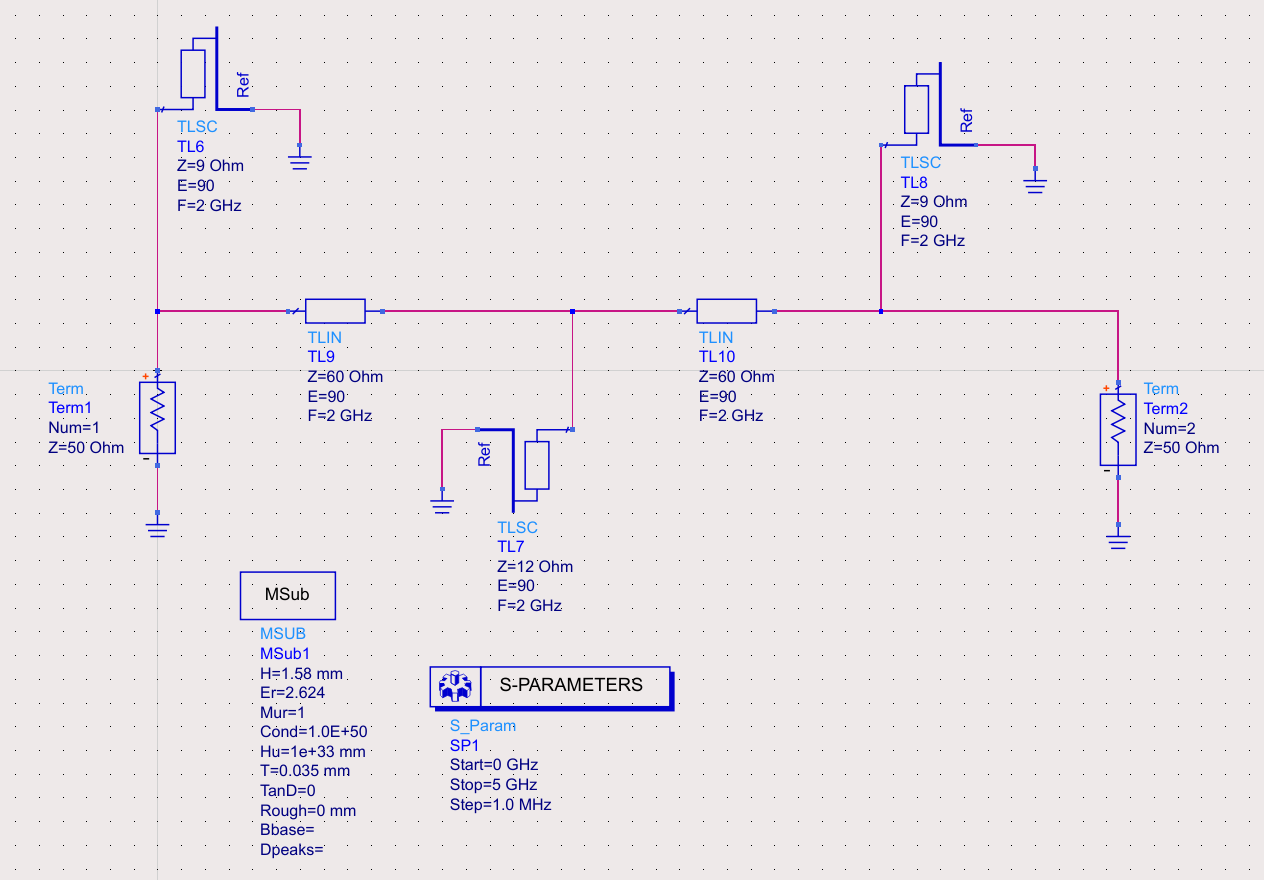
\includegraphics[width=0.7\linewidth]{../4synthPBande/inverseur_impedance/montage_inverseur_ADS}
	\caption{Schéma passe bande micro-ruban lignes quart d'onde}
	\label{fig:montageinverseurads}
\end{figure}
\newpage
Après simulation en paramètres S et affichage du coefficient de transmission on obtient la figure suivante:
\begin{figure}[H]
	\centering
	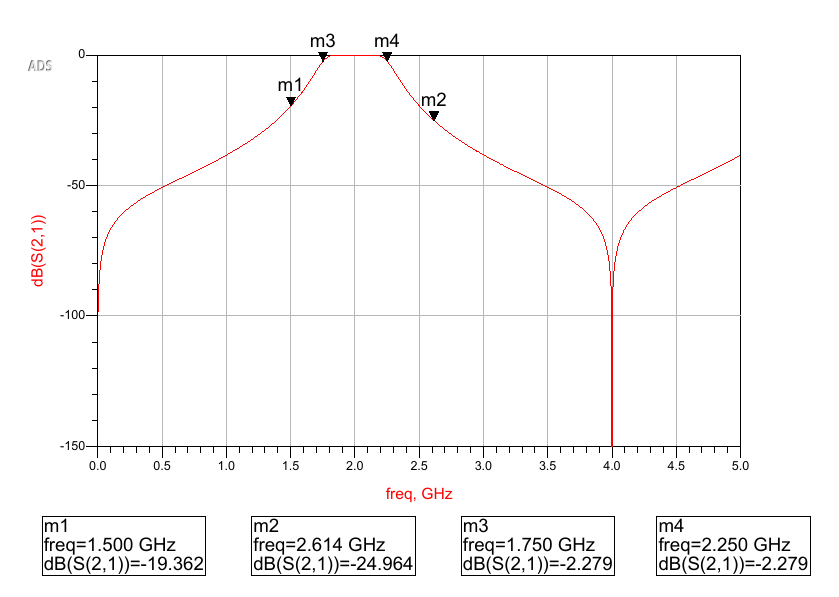
\includegraphics[width=0.7\linewidth]{../4synthPBande/inverseur_impedance/resultat_simulation}
	\caption{Simulation module de S21 passe bande micro-ruban lignes quart d'onde}
	\label{fig:resultatsimulation}
\end{figure}

Les points m1 et m2 permettent de valider la conformité aux fréquences de coupure avec une atténuation respective de 19,362dB et 24,964dB. Au contraire, la bande passante présente une atténuation anormalement supérieure de 2,1dB. Ce résultat ne remet pas en question la fonction passe bande mais l'écart présent n'est plus négligeable. Malheureusement aucune explication n'a été trouvé à ce problème. \\

Comme pour la synthèse précédente il est possible d'observer le domaine de validité de la fonction passe bande. Dans ce cas la bande valide s'étant de 0Hz à 4GHz. Cette valeur est deux fois supérieure à la synthèse précédente. C'est là l\emph{'avantage principal d'une conception à base uniquement de lignes quart d'onde.} Cela s'explique par la forme de la fonction tangente. Avec $l=\lambda/4$ donc $\beta l = \pi$ la ligne quart d'onde exploite la discontinuité de la fonction trigonométrique et donc deux périodes contre une seule pour la ligne demie onde. Un second phénomène intéressant est observable. La réponse fréquentielle présente une atténuation infinie à 4GHz. Il existe un montage appelé Dual Behavior Resonator (DBR)\footnote{On pensera au mnémotechnique Deux BièRes} basé sur deux stubs parallèles dont la longueur totale vaut $\lambda/4$ permettant de profiter à la fois de la fonction passe bande mais aussi de placer un zéro de transmission à l'endroit souhaité. Cette innovation est issue des laboratoires français. 
\newpage
\section{Synthèse d'un amplificateur à bande étroite}
L’objectif de cette partie est de réaliser un amplificateur à bande étroite adapté en MAG (Maximum Available Gain) à 2GHz prenant la méthodologie de conception (vue en TD). Le transistor utilisé est le transistor AT-41485. En entrée, il reçoit le maximum de puissance par le générateur, et à la sortie, il envoie le maximum de puissance à la charge de 50 Ohm.

\subsection{Démarche de conception d’un amplificateur}
\subsubsection{Théorie de la matrice S}
Les paramètres S relient les ondes réfléchies et les ondes incidentes. En mathématiques, la matrice S est utilisée pour représenter ces paramètres. Un quadripôle est illustré à la figure \ref{fig:matrice_s}, les entrées sont représentées par $a_{1}$ et $a_{2}$, les sorties sont représentées par $b_{1}$ et $b_{2}$. 

\begin{figure}[H]
	\centering
	\includegraphics[width=0.9\linewidth]{../5SynthAmp/Matrice_S}
	\caption{Matrice S dans un quadripôle}
	\label{fig:matrice_s}
\end{figure}

La matrice de ce quadripôle est la suivante :

\begin{equation}
	\begin{bmatrix}
		b_{1}\\
		b_{2}
	\end{bmatrix}
	=
	\begin{bmatrix}
		S_{11} & S_{12}\\
		S_{21} & S_{22}
	\end{bmatrix}
	\begin{bmatrix}
		a_{1}\\
		a_{2}
	\end{bmatrix}
\end{equation}

En développant cette matrice, on obtient la relation suivante :

\begin{equation}
	\left\{\begin{matrix}
		b_{1}=S_{11}a_{1}+S_{12}a_{2}\\
		b_{2}=S_{21}a_{1}+S_{22}a_{2}
	\end{matrix}\right.
	\label{eqmatrix}
\end{equation}

D’où:

$\bullet$ $S_{11}$: Le coefficient de réflexion à l’entrée lorsque la sortie du quadripôle est fermée sur une charge adaptée;

$\bullet$ $S_{12}$: Le coefficient de transmission entre le port 2 et le port 1 lorsque le port 1 est fermée sur une charge adaptée;

$\bullet$ $S_{21}$: Le coefficient de transmission entre le port 1 et le port 2 lorsque le port 2 est fermée sur une charge adaptée;

$\bullet$ $S_{22}$: Le coefficient à la sortie du quadripôle.

\subsubsection{Calcul du MAG}

Le transistor AT-41485 est défini par les paramètres de la matrice S. Grâce à la datasheet, nous pouvons obtenir les paramètres S de AT-41485, c'est-à-dire les éléments de la matrice S. Selon le cahier des charges, l'amplificateur à concevoir fonctionnera à 2GHz, et le point de polarisation retenu pour l’amplificateur est le suivant :

{\centering
	$V_{CE}=8V$\\
	$I_{C}=10mA$\\
}

Donc la datasheet choisie est la suivante: 
\begin{figure}[H]
	\centering
	\includegraphics[width=0.9\linewidth]{../5SynthAmp/Datasheet_AT41485}
	\caption{Paramètres S du transistor AT-41485 issue de la datasheet}
	\label{fig:datasheet_AT}
\end{figure}

Les paramètres S de AT-41485 sont :

{\centering
$S_{11}=0.58e^{j166^{\circ}}$\\
$S_{21}=3.55e^{j64^{\circ}}$\\
$S_{12}=0.06e^{j54^{\circ}}$\\
$S_{22}=0.41e^{-j38^{\circ}}$\\
}

Pour réaliser cet amplificateur, il faut mettre en cascade. Donc on insère le transistor polarisé entre deux quadripôles sans pertes symétriques : Quadripôle d’entrée et quadripôle de sortie. La figure \ref{fig:schema_ampli} montre le montage amplificateur. 
\begin{figure}[H]
	\centering
	\includegraphics[width=0.9\linewidth]{../5SynthAmp/Schema_ampli}
	\caption{Schéma quadripôle du montage amplificateur}
	\label{fig:schema_ampli}
\end{figure}

La matrice S du quadripôle d’entrée est :
\begin{equation}
	Q_{E} = \begin{bmatrix}
		\Gamma_{E} & t_{E}\\
		t_{E} & \Gamma_{E}\\
	\end{bmatrix}
\end{equation}

La matrice S du quadripôle de sortie est :
\begin{equation}
	Q_{L} = \begin{bmatrix}
		\Gamma_{L} & t_{L}\\
		t_{L} & \Gamma_{L}\\
	\end{bmatrix}
\end{equation}

Parce que les quadripôles d'entrée et de sortie sont sans perte, la relation est la suivante :
\begin{equation}
	{\begin{bmatrix}
		S^\ast 
	\end{bmatrix}}'
	\begin{bmatrix}
		S
	\end{bmatrix}=
	\begin{bmatrix}
		I
	\end{bmatrix}
\end{equation}

Donc:
\begin{equation}
	\begin{bmatrix}
		\Gamma_{E}^\ast & t_{E}^\ast\\
		t_{E}^\ast & \Gamma_{E}^\ast
	\end{bmatrix}
	\begin{bmatrix}
		\Gamma_{E} & t_{E}\\
		t_{E} & \Gamma_{E}
	\end{bmatrix}=
	\begin{bmatrix}
		1 & 0\\
		0 & 1
	\end{bmatrix}
\end{equation}

Soit:
\begin{equation}
	\Gamma_{E}^{\ast}\Gamma_{E}+t_{E}^{\ast}t_{E}
	={\mid \Gamma_{E}\mid}^2+{\mid t_{E}\mid}^2
	=1
	\label{eq2}
\end{equation}

De même, on a:
\begin{equation}
	{\mid \Gamma_{L}\mid}^2+{\mid t_{L}\mid}^2
	=1
	\label{eq3}
\end{equation}

Ensuite, on utilise le graphe de fluence pour analyser la relation entre les trois parties de l'amplificateur. Par la mise en cascade du générateur, du quadripôle d’entrée, du transistor, du quadripôle de sortie, et de la charge, on peut déduire le graphe de fluence global comme suit :

\begin{figure}[H]
	\centering
	\includegraphics[width=0.9\linewidth]{../5SynthAmp/flux_global}
	\caption{Graphe de fluence global du montage amplificateur}
	\label{fig:flux_global}
\end{figure}

On suppose que le générateur et la charge sont adaptées, c’est-à-dire $\Gamma_{g}=\Gamma_{2}=0$, on peut simplifier le graphe de fluence comme suit :

\begin{figure}[H]
	\centering
	\includegraphics[width=0.9\linewidth]{../5SynthAmp/flux_simple}
	\caption{Graphe de fluence simplifié du montage amplificateur}
	\label{fig:flux_simple}
\end{figure}

Grâce aux équations \ref{eqmatrix}, nous pouvons obtenir la relation suivante:
\begin{equation}
	b_{2}=\frac{S_{21}}{1-S_{22}\Gamma_{L}}a_{1}
\end{equation}

Soit: 
\begin{equation}
	b_{1}=S_{11}a_{1}+\frac{S_{12}S_{21}\Gamma_{L}}{1-S_{22}\Gamma_{2}}a_{1}
\end{equation}

Par conséquent, nous pouvons dériver l'equation de ${S_{11}}'$:
\begin{equation}
	{S_{11}}'=\frac{b_{1}}{a_{1}}
	=S_{11}+\frac{S_{12}S_{21}\Gamma_{L}}{1-S_{22}\Gamma_{L}}
\end{equation}

De la même manière, nous pouvons dériver l'equation de ${S_{22}}'$:
\begin{equation}
	{S_{22}}'=\frac{b_{2}}{a_{2}}
	=S_{22}+\frac{S_{12}S_{21}\Gamma_{E}}{1-S_{11}\Gamma_{E}}
\end{equation}

On peut utiliser la règle de Mason afin de déterminer le gain de l’amplificateur. Cette règle indique que :
\begin{equation}
	G=\frac{B}{A}=\frac{N}{D}
\end{equation}

Où:
\begin{equation}
	\left\{\begin{matrix}
		D=1-\sum{B_{i}}+\sum{B_{i}B_{j}}-\sum{B_{i}B_{j}B_{k}}+{\cdots}\\ 
		N=\sum{T_{i}D_{i}}
	\end{matrix}\right.
\end{equation}

Avec:

$\bullet$ $B_{i}$ représente le produit des paramètres S dans une boucle;\\
$\bullet$ $B_{i}B_{j}$ est les produits des boucles disjointes ;\\
$\bullet$ $T_{i}$ est le produit des paramètres S d’un trajet direct de A à B;\\
$\bullet$ $D_{i}$ est calculé comme D après avoir supprimé le trajet direct de A à B.\\

Donc dans nos cas, on obtient finalement:
\begin{equation}
	G=\frac{N}{D}=\frac{t_{e}S_{21}t_{L}}{1-\left (S_{11}\Gamma_{e}+S_{22}\Gamma_{L}+S_{21}\Gamma_{L}S_{12}\Gamma_{e}\right)+S_{11}\Gamma_{e}S_{22}\Gamma_{L}}
\end{equation}

Par la suite, on utilise les équations \ref{eq2} et \ref{eq3} pour remplacer $\mid t_{e}\mid ^{2}$ et $\mid t_{l}\mid ^{2}$. On obtient donc:
\begin{equation}
	G_{T}=\frac{\mid t_{e}\mid ^{2}}{\mid 1-\Gamma_{e}{S_{11}}'\mid ^{2}}\mid S_{21}\mid ^{2}\frac{\mid t_{L}\mid ^{2}}{\mid 1-\Gamma_{L}S_{22}\mid^{2}}
\end{equation}

Pour connaître le gain maximum de l’amplificateur, on suppose que le quadripôle d’entrée adapte en puissance l’entrée du transistor au générateur et que le quadripôle de sortie adapte la sortie du transistor à la charge, alors :
\begin{equation}
	\Gamma_{e}={S_{11}}'^\ast
\end{equation}
\begin{equation}
	\Gamma_{L}={S_{22}}'^\ast
\end{equation}

Etant donné que les paramètres $S_{11}$, $S_{21}$, $S_{12}$, et $S_{22}$ sont connus, seuls ${S_{11}}'$ et ${S_{22}}'$ sont inconnus, ce qui nous donne deux équations :
\begin{equation}
	\left\{\begin{matrix}
		{S_{11}}'=\cfrac{B_{1}+\sqrt{B_{1}^{2}-4\mid C_{1}\mid^{2}}}{2{C_{1}}^\ast}\\
		{S_{22}}'=\cfrac{B_{2}+\sqrt{B_{2}^{2}-4\mid C_{2}\mid^{2}}}{2{C_{2}}^\ast}
	\end{matrix}\right.
\end{equation}

Avec:
\begin{equation}
	\left\{\begin{matrix}
		B_{1}=1+\mid S_{11}\mid^{2}-\mid S_{22}\mid^{2}-\mid \Delta \mid^{2}\\
		B_{2}=1+\mid S_{22}\mid^{2}-\mid S_{11}\mid^{2}-\mid \Delta \mid^{2}\\
		C_{1}=S_{11}-\left(\Delta S_{22}^\ast\right)\\
		C_{2}=S_{22}-\left(\Delta S_{11}^\ast\right)\\
		\Delta=S_{11}S_{22}-S_{12}S_{21}
	\end{matrix}\right.
\end{equation}

Par application numérique, on obtient:

{\centering
$\Delta=0.047e^{j182^{\circ}}$, $B_{1}=1.166$, $B_{2}=0.829$,\\ $C_{1}=0.57e^{j165^{\circ}}$, $C_{2}=0.39e^{-j41^{\circ}}$,\\ $S_{11}'=0.799e^{j164^{\circ}}$, $S_{22}'=0.725e^{-j41^{\circ}}$\\
}

Le gain MAG obtenu a donc la forme suivante :
\begin{equation}
	MAG=\frac{1}{\mid 1-\mid S_{11}'\mid^{2}\mid^{2}}\mid S_{21}\mid^{2}\frac{1-\mid S_{22}'\mid^{2}}{\mid 1-S_{22}S_{22}'^{\ast}\mid^{2}}
\end{equation}

En utilisant les valeurs calculées ci-dessus, en appliquant cette équation, on peut obtenir:

{\centering
	$MAG=13.58 dB$ pour $S_{12}=0$\\
}

\subsubsection{Vérification de la stabilité de l’amplificateur}
Il convient de vérifier la stabilité de l’amplificateur dans ces deux conditions:

{\centering
$\mid \Delta\mid<1$\\
$k>1$\\
}

Par les calculs précédents, on a obtenu:

{\centering
$\Delta=0.047e^{j182^{\circ}}=-0.046-j0.001$\\
}

Ensuite, on peut calculer $k$ utilisant cette equation:
\begin{equation}
	k=\frac{1+\mid \Delta\mid^{2}-\mid S_{11}\mid^{2}-\mid S_{22}\mid^{2}}{2\mid S_{11}\mid \mid S_{22}\mid}
\end{equation}

Donc on obtient:

{\centering
	$k=1.168$\\
}

Ces deux résultats remplissent les conditions de stabilité de l'amplificateur. Donc il prouve la stabilité de notre transistor à 2GHz.


\subsection{Conception d’amplificateur idéal}
Après avoir préalablement calculé le MAG, dans un premier temps il s’agit de concevoir l’amplificateur avec la ligne idéal. Cette conception est mise en œuvre avec le logiciel ADS en utilisant le modèle de transistor AT-41485 qui est déjà polarisé.

Pour obtenir le MAG de l’amplificateur en bande étroite, il faut adapter l’entrée et la sortie du transistor, donc on va utiliser une adaptation simple stub adaptée. En entrée, le transistor présent un coefficient de réflexion égal à $S_{11}’$ qui doit être adapté à l’impédance du générateur (en général 50 Ohm). Il présente, en sortie, un coefficient de réflexion égal à $S_{22}’$ qui doit être adapté à l’impédance de la charge (en général 50 Ohm). La structure est la suivante :

\begin{figure}[H]
	\centering
	\includegraphics[width=0.6\linewidth]{../5SynthAmp/adaptation_e_s}
	\caption{Schéma d'adaptation du  transistor}
	\label{fig:adaptation_e_s}
\end{figure}

On sait que le coefficient de réflexion en entrée est égal à:
\begin{equation}
	S_{11}'=0.799e^{j164^{\circ}}=-0.7699+j0.2140
\end{equation}

Grâce à l’Abaque de Smith, on obtient les longueurs de stub en entrée suivantes:

{\centering
	$d_{1}=0.192\lambda$\\
	$l_{1}=0.029\lambda$\\
}
	
D’où $d_{1}$ et $l_{1}$ sont respectivement exprimés par la figure suivante:
\begin{figure}[H]
	\centering
	\includegraphics[width=0.55\linewidth]{../5SynthAmp/simple_stub_e}
	\caption{Schéma adaptation simple stub en entrée du transistor}
	\label{fig:simple_stub_e}
\end{figure}

De la même manière, on peut obtenir les longueurs de stub en sortie suivantes :
 
{\centering
	$d_{2}=0.321\lambda$\\
	$l_{2}=0.133\lambda$\\
}

En utilisant ces 4 paramètres sous ADS, le montage de l’amplificateur avec les lignes idéales est montrée dans la figure \ref{fig:ligne_ideal}:
\begin{figure}[H]
	\centering
	\includegraphics[width=0.7\linewidth]{../5SynthAmp/ligne_ideal}
	\caption{Schéma de l’amplificateur avec les lignes idéales}
	\label{fig:ligne_ideal}
\end{figure}

Le montage qu’on a utilisé représente le résultat de la simulation ci-dessous (Dans cette simulation, S12 peut être approximativement égal à 0) :
\begin{figure}[H]
	\centering
	\includegraphics[width=1\linewidth]{../5SynthAmp/ligne_ideal_Sparametres}
	\caption{Simulation module de S montage avec ligne idéal en dB}
	\label{fig:ligne_ideal_Sparametres}
\end{figure}

Lorsque la fréquence de simulation est de 2 GHz, les résultats montrent que $S_{21}$ est de 15.232 à ce point, c'est-à-dire que le MAG à ce moment est de 15.232 dB. Ce résultat est conforme à l'exigence du cahier des charges selon laquelle le MAG doit respecter 13.58 dB à 2 GHz. De plus, les réflexions d’entrée et de sortie qui représentées respectivement par le $S_{11}$ et le $S_{22}$ sont minimales à environ 2 GHz avec les valeurs -31.193 dB et -47.544 dB. Cela montre également que le transistor est adapté en entrée et en sortie.

Cependant, les valeurs numériques de ces longueurs ne sont pas figées. Lorsque la fréquence de travail change, la valeur de la longueur de simple stub change également en conséquence, et la valeur peut être calculée en appliquant l’Abaque de Smith.

\subsection{Conception d’amplificateur en technologie micro-ruban}
Après avoir montré le résultat de l’amplificateur avec les lignes idéal précédemment, dans cette partie, on va utiliser les lignes en technologie micro-ruban pour simuler une situation plus réaliste sous ADS.

Le substrat utilisé est téflon. D'après l'analyse des sections précédentes, dans cette partie on va fixer à 2 GHz la valeur de la constante diélectrique $\varepsilon_{r}$ est de 2.61 $F.m^{-1}$, et sur un modèle de substrat sans pertes, la tangente de perte $\mbox{tan}(\delta)$ est négligé.

L’outil LineCal fournie par le logiciel ADS peut déterminer les paramètres de substrat. Les longueurs $d_{1}$, $l_{1}$, $d_{2}$ et $l_{2}$ de la ligne idéale précédentes sont présentées par $L$ et $W$ de la ligne micro-ruban. Après avoir fixé $\varepsilon_{r}=2.61$, $h=1.58 mm$ et $f=2 GHz$, on peut calculer les valeurs de L et W. Les resultats sont comme suivant :

\begin{table}[H]
	\centering
	\begin{tabular}{|c|c|c|}
		\hline
		Composant & L (mm) & W(mm) \\
		\hline
		TL7 & 19.508 & 4.361 \\
		\hline
		TL5 & 2.946 & 4.361 \\
		\hline
		TL6 & 13.513 & 4.361 \\
		\hline
		TL8 & 32.615 & 4.361\\
		\hline
	\end{tabular}
	\caption{Tableau présentant les valeurs de L et W de la ligne micro-ruban}
\end{table}

On a appliqué ces valeurs à l'amplificateur, le schéma est présenté ci-dessous :
\begin{figure}[H]
	\centering
	\includegraphics[width=1.0\linewidth]{../5SynthAmp/ligne_micro_ruban}
	\caption{Schéma de l’amplificateur avec les lignes micro-ruban}
	\label{fig:ligne_micro_ruban}
\end{figure}
\newpage
Le montage qu’on a utilisé représente le résultat de la simulation ci-dessous:
\begin{figure}[H]
	\centering
	\includegraphics[width=1\linewidth]{../5SynthAmp/ligne_micro_ruban_Sparametres}
	\caption{Simulation module de S du montage avec ligne micro-ruban en dB}
	\label{fig:ligne_micro_ruban_Sparametres}
\end{figure}

Lorsque la fréquence de simulation est de 2 GHz, les résultats montrent que $S_{43}$ est de 15.232 à ce point, c'est-à-dire que le MAG à ce moment est de 15.232 dB, et ce résultat est également conforme à l'exigence du cahier des charges. De plus, les réflexions d’entrée et de sortie qui représentées respectivement par le $S_{33}$ et le $S_{44}$ sont minimales à environ 2 GHz avec les valeurs -31.194 dB et -47.549 dB. Les résultats sont cohérents avec ceux obtenus par le montage avec la ligne idéale.

\subsection{Adaptation d’un transistor avec polarisation}
Dans les sections précédentes, nous avons utilisé un modèle de transistor AT-41485 polarisé, qui satisfait déjà ces deux conditions :$V_{CE}=8 V$ et $I_{C}=10 mA$. Maintenant, on s’intéresse à la polarisation du transistor. La valeur de résistance de la résistance doit être calculée pour que le circuit réponde aux conditions de conception du transistor. Le circuit de polarisation à concevoir doit avoir une faible impédance pour les basses fréquences et une haute impédance pour les hautes fréquences. De plus, des condensateurs doivent être ajoutés entre le transistor et la source et la charge, respectivement, pour empêcher le courant continu d'entrer dans le reste du circuit.

La maquette donnée comporte le transistor à caractériser, sa polarisation et des lignes d'accès à la base et au collecteur d'une longueur électrique supérieure à $\lambda/2$ à 2 GHz. De plus, on dispose d'une ligne 50Ohm de traversée(THRU) et d’une ligne terminée par un court-circuit dans le plan d'entrée du transistor(REFLECT) qui permettent d'étalonner le relevé des paramètre S. La polarisation est découplée du signal par une ligne $\lambda/4$ a haute impédance et une capacité de retour à la masse sur les accès base et collecteur. 
\newpage

Le circuit est présenté ci-dessous:
\begin{figure}[H]
	\centering
	\includegraphics[width=0.75\linewidth]{../5SynthAmp/polarisation}
	\caption{Schéma de polarisation du transistor}
	\label{fig:polarisation}
\end{figure}

Après simulation, on peut obtenir les résultats suivants:
\begin{figure}[H]
	\centering
	\includegraphics[width=0.8\linewidth]{../5SynthAmp/polarisation_Sparametres}
	\caption{Simulation module de S du montage de polarisation du transistor en dB}
	\label{fig:polarisation_simu}
\end{figure}

Lorsque la fréquence de simulation est de 2 GHz, les résultats montrent que $S_{21}$ est de 18.437 à ce point, c'est-à-dire que le MAG à ce moment est de 18.437 dB. Ce résultat est conforme à l'exigence du cahier des charges. Cela montre également que le transistor est bien polarisé.


\newpage
\section{Conclusion}
Au cours de ce rapport il a été vu dans un premier temps une méthodologie de caractérisation d'une ligne micro-ruban sur divers diélectriques. La méthode consistait à la superposition entre les valeurs réelles expérimentales et celles obtenues à partir d'une modélisation. La réalisation d'une bonne caractérisation réside dans la complexité du modèle théorique, qui se doit être la plus réaliste possible. C'est ce qui a été mis en place à l'aide de la prise en compte de phénomènes physiques comme les discontinuités. Il est indispensable de réaliser cette étape de caractérisation avant toutes réalisations de fonctions électroniques car il faut avoir connaissance des paramètres du diélectrique pour que les simulations effectuées soient proches de ce qu'on obtiendrait lors de la réalisation en laboratoire.\\
Le filtre passe-bas elliptique a été conçu en essayant de respecter au mieux les exigences du cahier des charges. Une telle conception a également permis d'étudier un tout nouveau type de filtre qu'est le filtre elliptique, autrement appelé filtre de Cauer. La conception en éléments localisés a été réalisée avec les mêmes méthodes employées lors de la conception en moyennes fréquences. La seconde partie consistait à la transposition en technologie micro-ruban. Un tel passage s'appui sur un modèle physique basé sur des hypothèses. La réalisation impose de fixer des paramètres géométriques choisis en fonction des contraintes concepteurs (contraintes technologiques photolithographies). Les simulations ont montré que les hypothèses ne sont pas toujours respectées. Il s'agit là d'une leçon utile pour notre future carrière d'ingénieur. En effet, les projets imposent parfois de faire des hypothèses, l'enjeu est de savoir si elles sont bien applicables dans le contexte donné.\\
La conception d'un filtre passe bande a été présentée suivant différentes étapes. La première s'attache à vérifier et, si nécessaire, recentrer le gabarit. La suivante opère une transformation du gabarit en passe bas. Cela rend plus aisé le calcul de l'ordre et des valeurs normalisées. Viens ensuite l'étape de dénormalisation visant à remplacer chaque composant réactif en résonateur LC série ou parallèle. Le résultat de cette synthèse peut être simulé pour valider le bon fonctionnement. Dans notre cas, une dissymétrie lors du recentrage couplée à un ordre de filtre limite ont entraînés une légère sortie du gabarit. L'étape finale de transposition en technologie micro-ruban est spécifique aux contraintes hautes fréquences. Elle vise à transposer les résonateurs LC en ligne micro-ruban. Deux approches ont été présentées : la première basée uniquement sur des lignes demie onde et la seconde sur des lignes quart d'onde. Dans les deux cas la méthode est similaire, trouver un modèle équivalant aux résonateurs série et parallèle pour opérer la transposition technologique. Finalement, nous avons pu monter par simulation que la bande de validité de la fonction passe bande est deux fois plus large pour la synthèse à base de lignes quart d'onde que pour celle basée sur des lignes demie onde.\\
La dernière partie présente la conception d'une fonction d'électronique : l'amplification. Il s'agissait de travailler avec un transistor AT-41485 faible bruit pour amplifier le signal à 2 GHz. De la même manière qu'en électronique des basses ou moyennes fréquences, il a été nécessaire de polariser le transistor. Sa matrice S varie en fonction de la polarisation et de la fréquence ce qui complique la mise au point d'amplificateurs en hautes fréquences. En effet, dans un cas réel, une polarisation n'est jamais parfaite et un petit écart sur la tension $V_{CE}$ ou le courant $I_C$ peut changer brutalement la matrice $S$. Il a donc été nécessaire de déterminer les paramètres S avant la conception des quadripôles d'entrée et de sortie pour adapter.\\

Ce TP traitant d’une thématique concrète a suscité notre intérêt. Les quatre étudiants, conscients des nombreuses connaissances acquises par ce travail, sont satisfaits de l'enseignement. Cela a même suscité des questionnements sur les choix de spécialités de cinquième année et peut-être des vocations. Nous souhaitons de nouveau remercier les enseignants qui ont su, par leur pédagogie, attiser notre curiosité.

La conception d'un filtre passe-bas de Tchebychef en hautes fréquences a été présentée suivant différentes étapes. La première étape était de faire une synthèse avec des éléments localisés. La seconde, de remplacer chaque élément localisé par des éléments distribués : des lignes de transmission. Après simulation, nous avons montré que l'ajout d'un stub avec des paramètres bien précis permet d'augmenter la plage de fréquences où la bande atténuée est conforme au cahier des charges. Ensuite, nous avons observé que l'utilisation d'un substrat en teflon est plus adapté aux hautes fréquences qu'un substrat epoxy. Pour finir, nous avons comparé le résultat de nos simulations avec des filtres déjà implémenté sur PCB. Bien que les allures des réponses en fréquences étaient semblables, des différences existaient liées principalement aux pertes du substrat non prise en compte dans notre simulation.









\newpage

\bibliography{bib_hf}{}
\bibliographystyle{plain}

\section*{Annexes}
\subsection*{Plaque avec lignes de caractérisation}
\includegraphics[scale=0.0525]{photo/ligne et filtre/plaque_caract_teflon.jpg}
\includegraphics[scale=0.07]{photo/ligne et filtre/plaque_caract_epoxy.jpg}
\begin{center}
	Annexe 1 : Photographies de plaques avec des lignes de caractérisation (à gauche plaque en verre téflon et à gauche en verre epoxy FR4)
\end{center}

\newpage
\subsection*{Code Octave (ou Matlab) pour calcul des g\_k puis des L\_k et C\_k}


\begin{lstlisting}frame=single] 
clear all;
close all;
clc;

% Calcul des coefficient g_k normalise pour un passe-bas avec une reponse de Tchebychiev
% L'attenuation maximal dans la bande passante sera de 0.1 dB

Amax = 0.1; % en dB
n = 5; % ordre du filtre
for k=1:n
a_k(k)=sin(((2*k - 1)* pi)/(2*n));
end

Beta = log(coth(Amax/17.37));
Gamma = sinh(Beta/(2*n));

for k=1:n   
b_k(k) = Gamma^2 + (sin((k*pi)/n))^2;
end


g_k(1) = (2*a_k(1))/Gamma;
for k=2:n
g_k(k) = (4 * a_k(k-1) * a_k(k)) / (b_k(k-1) * g_k(k-1));
end
g_k % Affichage des coefficient

fp = 2e9; % appele fc dans le poly de TP
R = 50;
Cdenorm = 1 / (2 * pi * fp * R);
Ldenorm =  R / (2 * pi * fp);
for k=1:n
if mod(k,2) ==0
C = g_k(k) * Cdenorm;
printf("C%d =%e\n",k, C);
else
L = g_k(k) * Ldenorm;
printf("L%d =%e\n",k, L);
end
end


\end{lstlisting}



\end{document}
